%%%%%%%%%%%%%%%%%%%%%%%%%%%%%%%%%%%%%%%%%
% Focus Beamer Presentation
% LaTeX Template
% Version 1.0 (8/8/18)
%
% This template has been downloaded from:
% http://www.LaTeXTemplates.com
%
% Original author:
% Pasquale Africa (https://github.com/elauksap/focus-beamertheme) with modifications by 
% Vel (vel@LaTeXTemplates.com)
%
% Template license:
% GNU GPL v3.0 License
%
% Important note:
% The bibliography/references need to be compiled with bibtex.
%
%%%%%%%%%%%%%%%%%%%%%%%%%%%%%%%%%%%%%%%%%

%----------------------------------------------------------------------------------------
%	PACKAGES AND OTHER DOCUMENT CONFIGURATIONS
%----------------------------------------------------------------------------------------

\documentclass{beamer}

\usetheme[numbering=fullbar]{focus} % Use the Focus theme supplied with the template
% Add option [numbering=none] to disable the footer progress bar
% Add option [numbering=fullbar] to show the footer progress bar as always full with a slide count

% Uncomment to enable the ice-blue theme
%\definecolor{main}{RGB}{92, 138, 168}
%\definecolor{background}{RGB}{240, 247, 255}

%------------------------------------------------

\usepackage{booktabs} % Required for better table rules

%----------------------------------------------------------------------------------------
%	 TITLE SLIDE
%----------------------------------------------------------------------------------------


\title{A maximum-flow model for digital elastica shape optimization}
\subtitle{DGMM 2021}

\author{  
  {Daniel Antunes\textsuperscript{1} \\ Jacques-Olivier Lachaud\textsuperscript{1} and \\ Hugues Talbot\textsuperscript{2}}
}
  
  
\date
  {25 May 2021}


\institute
  {
	\textsuperscript{1}LAMA, Université Savoie Mont Blanc \\ 
	\textsuperscript{2}CentraleSupélec, Université Paris-Saclay
  }

%\title{Focus: \\ A Minimalist Beamer Theme}
%
%\subtitle{Subtitle}
%
%\author{Author 1 \\ Author 2}

%\titlegraphic{\includegraphics[scale=1.25]{Images/focuslogo.pdf}} % Optional title page image, comment this line to remove it

%\institute{Institute Name \\ Institute Address}
%
%\date{dd mm yyyy}




\usepackage[utf8]{inputenc}
\usepackage[T1]{fontenc}
\usepackage[french,english]{babel}
\usepackage{graphicx}
\usepackage{caption,subcaption}
\usepackage{multirow}
\captionsetup{compatibility=false}

\usepackage[linesnumbered,commentsnumbered,ruled,vlined]{algorithm2e}
\usepackage[linewidth=2.5pt,linecolor=black,nobreak=true]{mdframed}
\mdfsetup{frametitlealignment=\center}

\usepackage{amstext,amsmath,amssymb,bm,bbm,graphicx,mathtools,accents}
\usepackage{tikz}
\usetikzlibrary{decorations.pathreplacing}
\usepackage{transparent}

\usepackage[style=authoryear,maxbibnames=99,maxcitenames=5,backref=true,backend=biber,citestyle=authoryear]{biblatex}
\AtBeginBibliography{\footnotesize}
\addbibresource{main.bib}

%%%%%%%  Environments  %%%%%%%%%%%

\newcounter{definition}[section]
\newenvironment{definition}[1]{\refstepcounter{definition} \par\bigskip \noindent  \begin{minipage}[b]{\linewidth} 
\textbf{Definition~\thedefinition(#1):}}{\end{minipage} \par\bigskip}

\newcounter{example}[section]
\newenvironment{example}{\refstepcounter{example} \par\medskip
\noindent  \begin{minipage}[b]{\linewidth} \textbf{Example~\theexample :}}{\end{minipage} \par\bigskip}

\newcounter{proposition}[section]
\newenvironment{proposition}[1]{\refstepcounter{proposition} \par\medskip \noindent  \begin{minipage}[b]{\linewidth} \textbf{Proposition~\theproposition(#1):}}{\end{minipage} \par\bigskip}

\newcounter{theorem}[section]
\newenvironment{theorem}[1]{\refstepcounter{theorem} \par\medskip \noindent  \begin{minipage}[b]{\linewidth} \textbf{Theorem~\thetheorem(#1):}}{\end{minipage} \par\bigskip}

\newenvironment{proof}{\noindent\ignorespaces\textit{Proof: }}{\hfill $\blacksquare$ \par\noindent\ignorespacesafterend\medskip}

\newcounter{assumption}[section]
\newenvironment{assumption}{ \refstepcounter{assumption} \renewcommand{\theequation}{A.\arabic{assumption}}}{\renewcommand{\theequation}{\arabic{section}.\arabic{equation}} }



%%%%%%%%%%%%%% Commands %%%%%%%%%%%
\newcommand{\daniel}[1]{{\color{black}{#1}}}
\newcommand{\revision}[1]{{\color{blue}{#1}}}

\newcommand{\transp}{\mathbf{T}}
\newcommand{\edge}[2]{ ( #1,#2 )}

\newcommand{\sketch}[1]{{\color{red}{#1}}}
\newcommand{\ol}[1]{{\overline{#1}}}
\newcommand{\av}[1]{\accentset{\circ}{\vec{#1}}}
\newcommand{\Ds}{D}
\newcommand\figTable[2]{\raisebox{-.5\height}{\includegraphics[scale=#1]{#2}}}


\DeclareMathOperator*{\argmin}{arg\,min}
\DeclareMathOperator*{\argmax}{arg\,max}
\renewcommand{\vec}[1]{\bm{#1}}
\DeclarePairedDelimiter\norm{\lVert}{\rVert}%
\DeclarePairedDelimiter\bignorm{\Big\lVert}{\Big\rVert}%
\DeclarePairedDelimiter\abs{\lvert}{\rvert}%

\newcommand{\GG}{ \mathcal{G}_{\vec{I}} }
\newcommand{\GGe}{ \mathcal{G}_{\vec{I}+} }
\newcommand{\GGc}[1]{ \mathcal{G}_C^{(#1)} }
\newcommand{\GGcc}{ \mathcal{G}_C}

\makeatletter
\DeclareFontFamily{U}{tipa}{}
\DeclareFontShape{U}{tipa}{m}{n}{<->tipa10}{}
\newcommand{\arc@char}{{\usefont{U}{tipa}{m}{n}\symbol{62}}}%

\newcommand{\arc}[1]{\mathpalette\arc@arc{#1}}

\newcommand{\arc@arc}[2]{%
  \sbox0{$\m@th#1#2$}%
  \vbox{
    \hbox{\resizebox{\wd0}{\height}{\arc@char}}
    \nointerlineskip
    \box0
  }%
}
\makeatother


%%%%%%%%%%% Misc %%%%%%%%%%%
\crefname{algocf}{alg.}{algs.}
\Crefname{algocf}{Algorithm}{Algorithms}
\Crefname{appsec}{Appendix}{Appendices}  

\setbeamertemplate{bibliography entry title}{}
\setbeamertemplate{bibliography entry location}{}
\setbeamertemplate{bibliography entry note}{}

\tikzset{
  invisible/.style={opacity=0},
  visible on/.style={alt={#1{}{invisible}}},
  alt/.code args={<#1>#2#3}{%
    \alt<#1>{\pgfkeysalso{#2}}{\pgfkeysalso{#3}} % \pgfkeysalso doesn't change the path
  },
}
 
\begin{document}
\captionsetup[subfigure]{labelformat=empty}

\begin{frame}
	\maketitle
\end{frame}

\begin{frame}{Outline}

\begin{enumerate}
	{
	\item{Motivation}
	\begin{itemize}
		\item{Image analysis tasks}		
		\item{Elastica energy and the completion property}	
		\item{Related works}
	\end{itemize}}
	\vspace{1em}
	\item{Proposed model}
	\begin{itemize}
		\item{Digital estimators}		
		\item{Curve-shortening flow}	
		\item{Elastica shape optimization}
		\item{Applications in imaging}			
	\end{itemize}
	\vspace{1em}
	\item{Conclusion and perspectives}
\end{enumerate}

\end{frame}

\section*{Motivation}
\subsection{Image analysis tasks \\[1em] Elastica energy and the completion property \\[1em] Related works}
\begin{frame}
{Image analysis tasks}

Let $I:\mathbb{Z}^2\rightarrow[0,1]^3$ a colored image.\\[1em]

\begin{minipage}[t][0.25\textheight][t]{0.5\textwidth}
\center
Segmentation\\

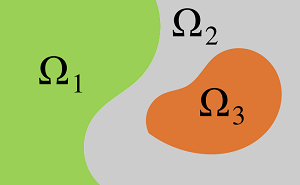
\includegraphics[scale=0.5]{figures/motivation/image-analysis/segmentation-stylised.png}
\end{minipage}%
\begin{minipage}[t][0.25\textheight][t]{0.5\textwidth}
\center
Inpainting\\


\includegraphics[scale=0.5]{figures/motivation/image-analysis/inpainting-stylised.png}
\end{minipage}%
%
\begin{align*}
 \argmin_{I^\star} &= \min_{I} Data(I) + Reg(I).
\end{align*}
%
Common geometric regularizers: perimeter, area.

\end{frame}
\subsection*{Elastica energy and the completion property}

\begin{frame}
{The elastica energy}

Let $X$ an Euclidean shape and $\alpha >0, \beta>0$.

\begin{align*}
 E(X) = \int_{\partial X}{ \alpha + \beta \kappa ^2ds}. 
\end{align*}


\end{frame}

\begin{frame}
{Completion property}
\begin{minipage}[t][0.45\textheight][t]{\textwidth}
\only<1->{
\center
$\min_{ X \subset \Omega } Data(X) + Perimeter(\partial X).$\\[1em]
}
\only<1>{
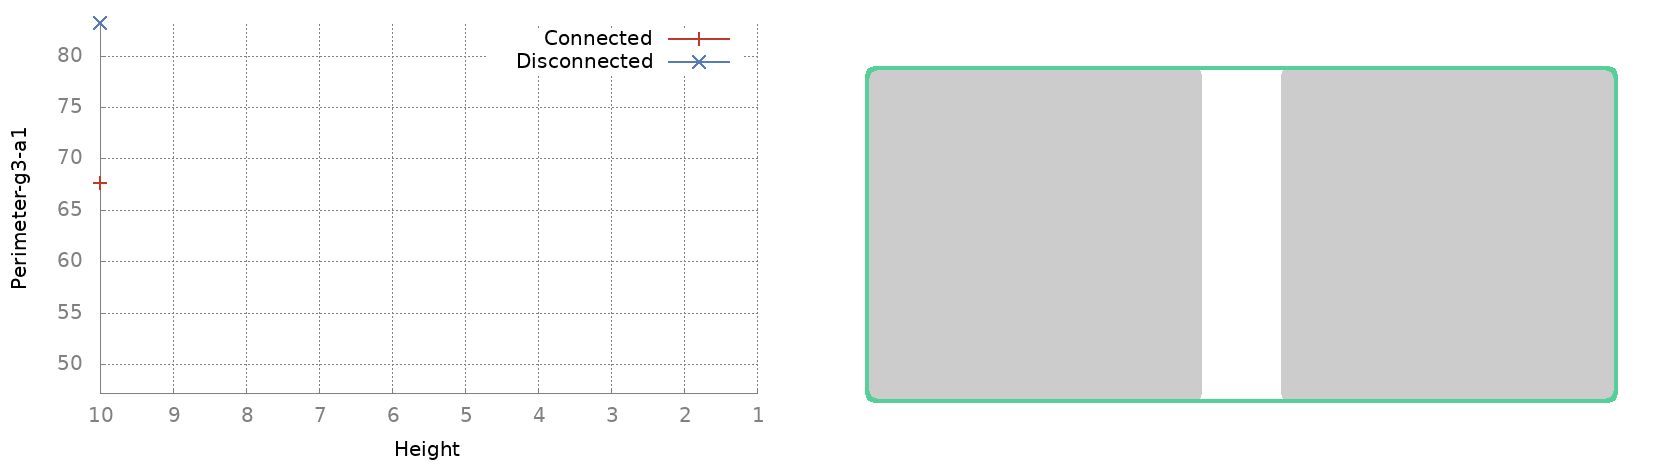
\includegraphics[scale=0.2]{figures/motivation/completion/perimeter-0.png}
}
\only<2>{
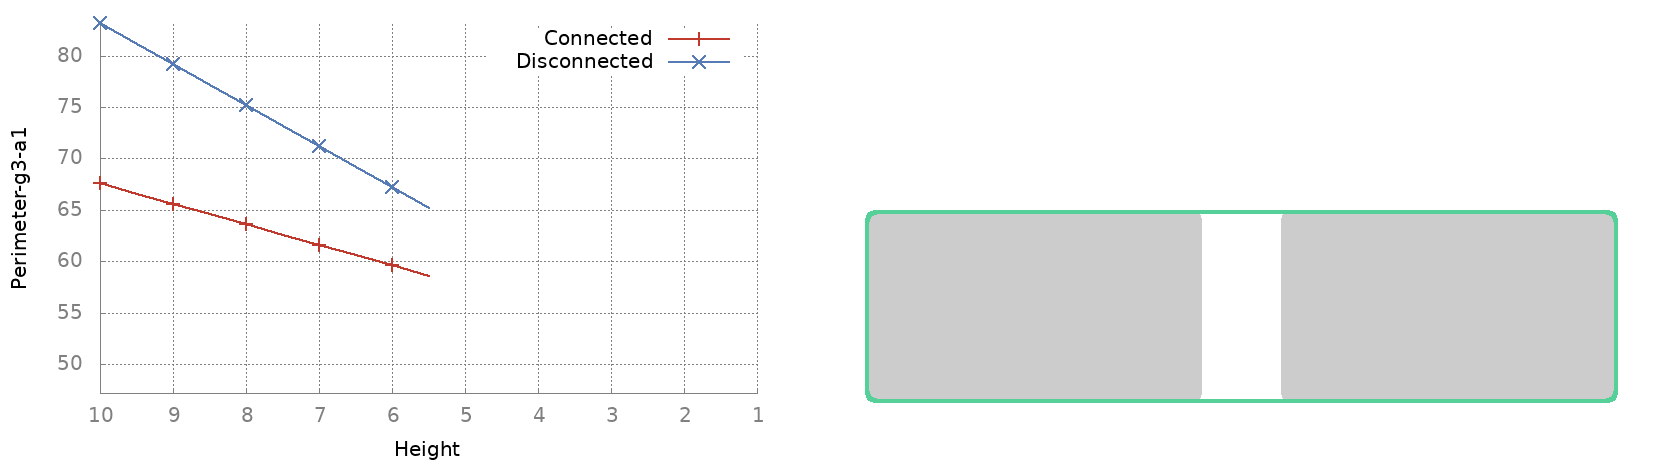
\includegraphics[scale=0.2]{figures/motivation/completion/perimeter-1.png}
}
\only<3>{
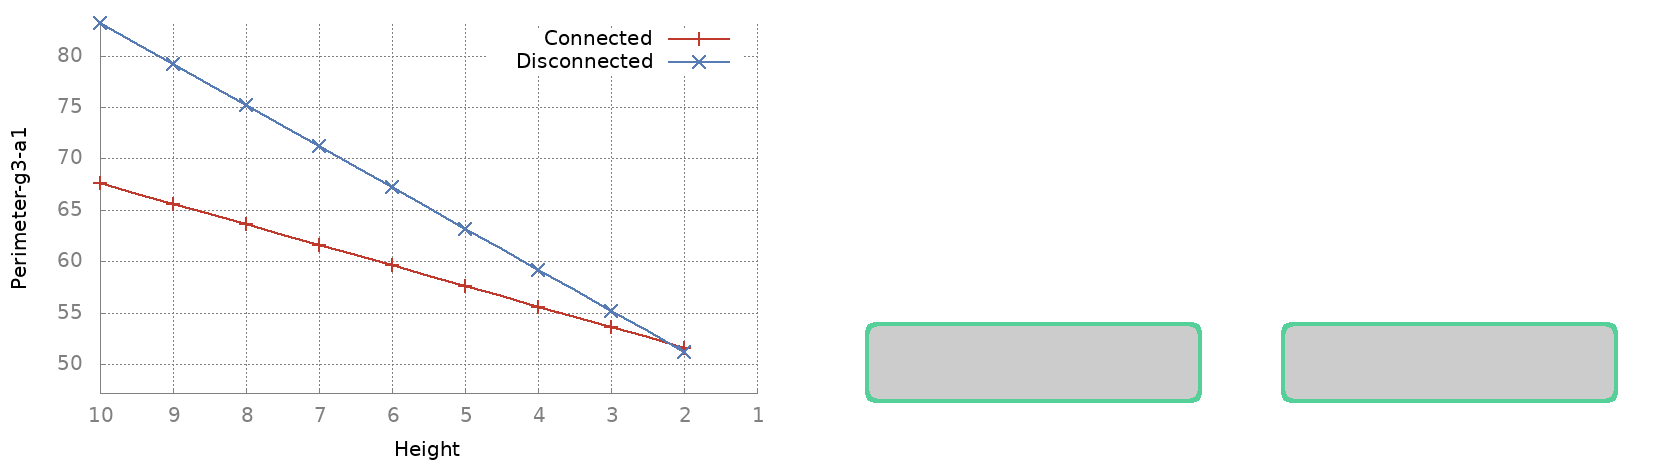
\includegraphics[scale=0.2]{figures/motivation/completion/perimeter-2.png}
}
\only<4->{
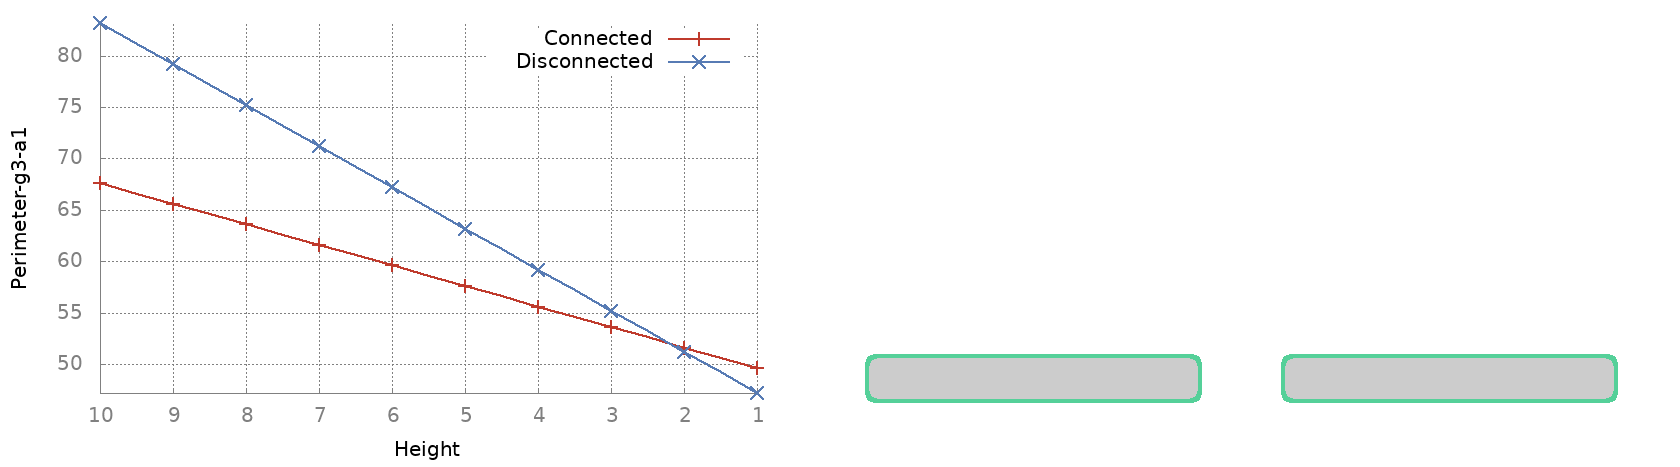
\includegraphics[scale=0.2]{figures/motivation/completion/perimeter-3.png}
}
\end{minipage}
\begin{minipage}[t][0.45\textheight][t]{\textwidth}
\only<5->{
\center
$\min_{ X \subset \Omega } Data(X) + Perimeter(\partial X) + Curvature^2(\partial X).$\\[1em]
}
\only<5>{
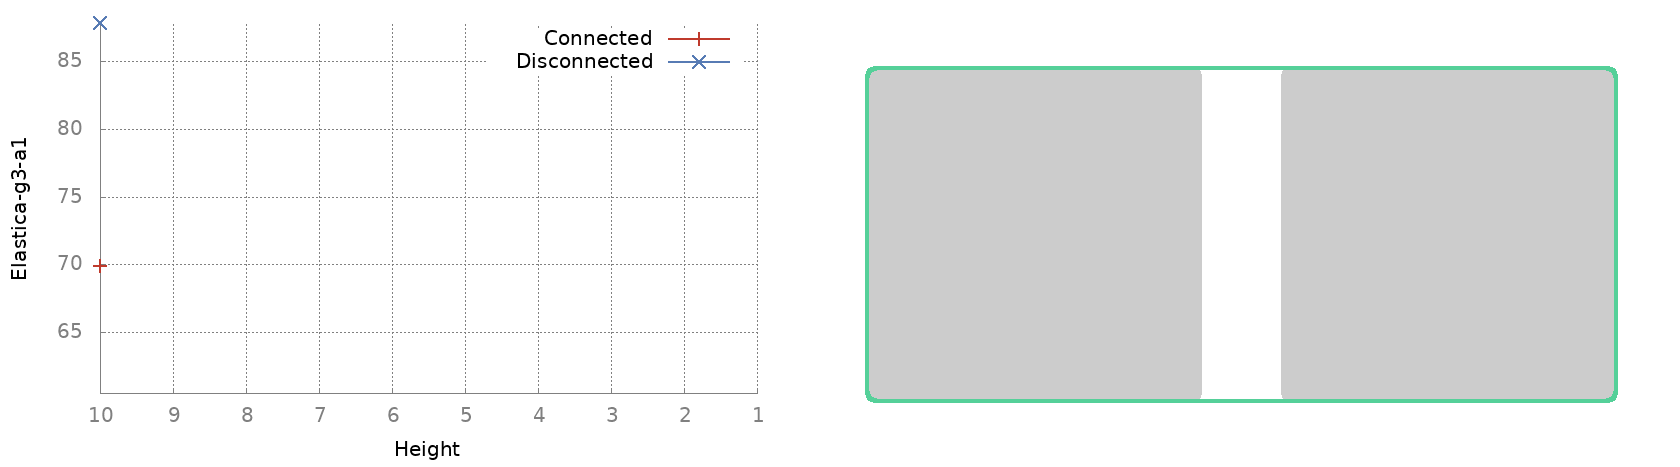
\includegraphics[scale=0.2]{figures/motivation/completion/elastica-0.png}
}
\only<6>{
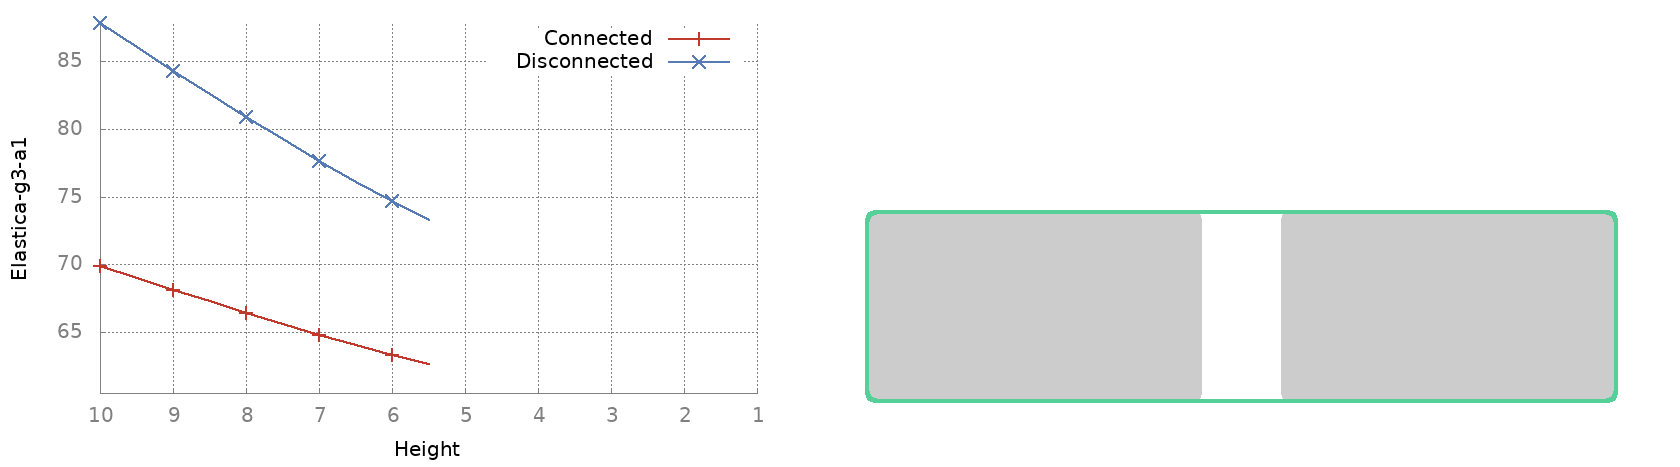
\includegraphics[scale=0.2]{figures/motivation/completion/elastica-1.png}
}
\only<7>{
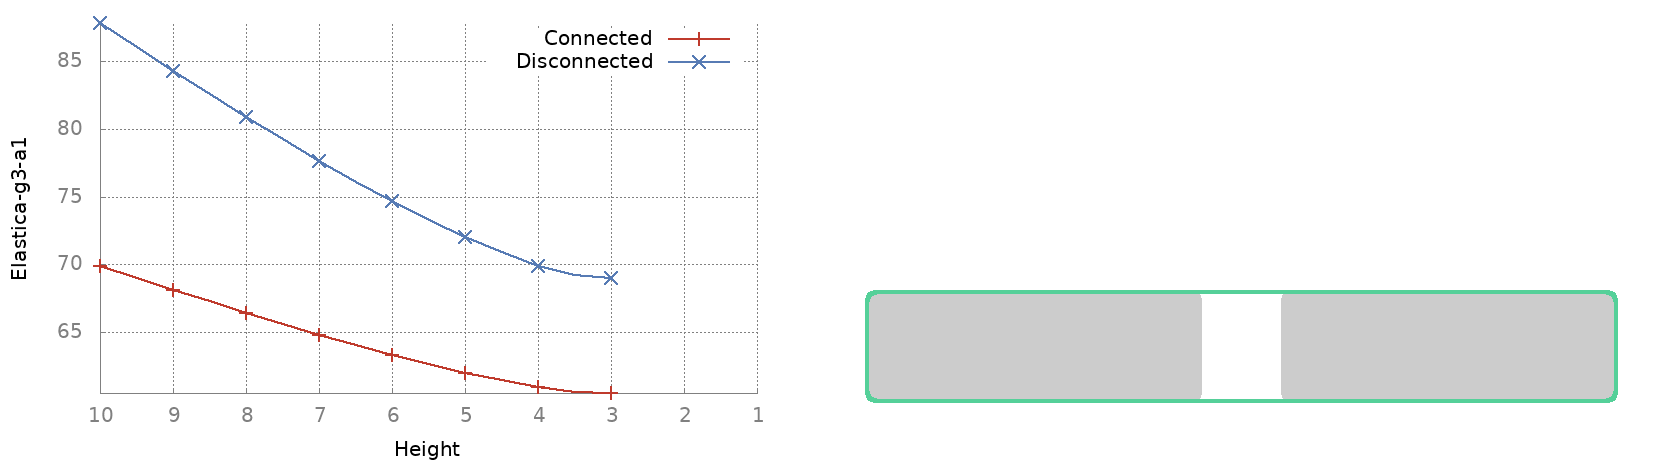
\includegraphics[scale=0.2]{figures/motivation/completion/elastica-2.png}
}
\only<8->{
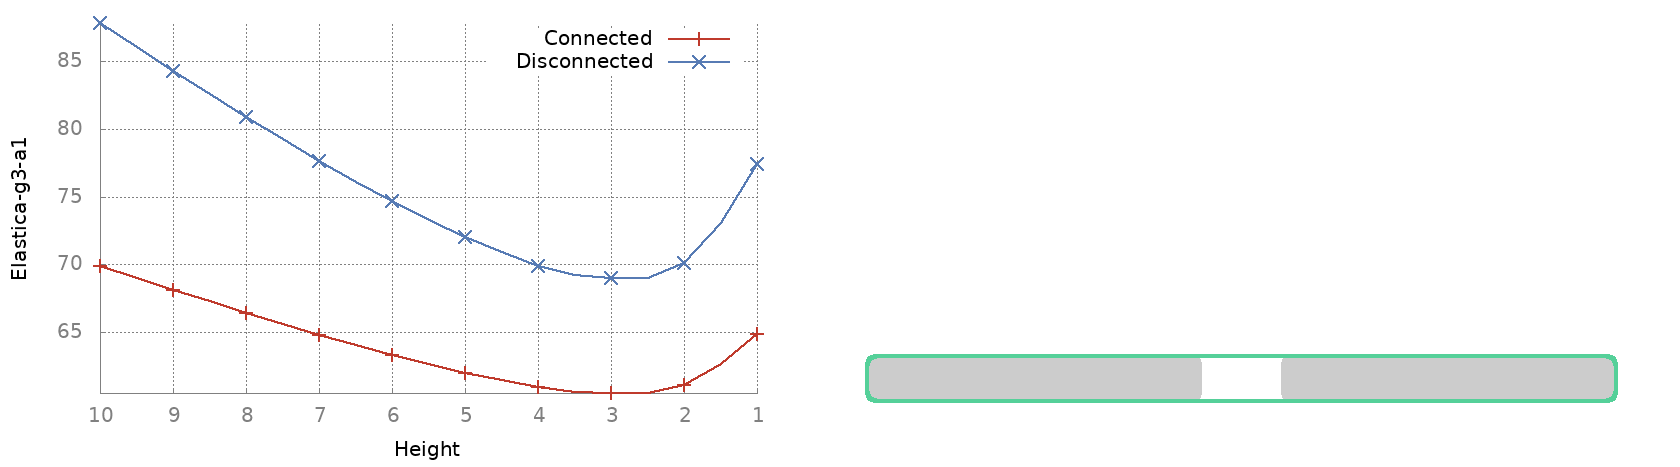
\includegraphics[scale=0.2]{figures/motivation/completion/elastica-3.png}
}
\end{minipage}
\end{frame}

\begin{frame}
{Completion property}
\begin{minipage}[t][0.45\textheight][t]{\textwidth}
\only<1->{
\center
$\min_{ X \subset \Omega } Data(X) + Perimeter(\partial X) + Curvature^2(\partial X).$\\[1em]
}
\only<1>{
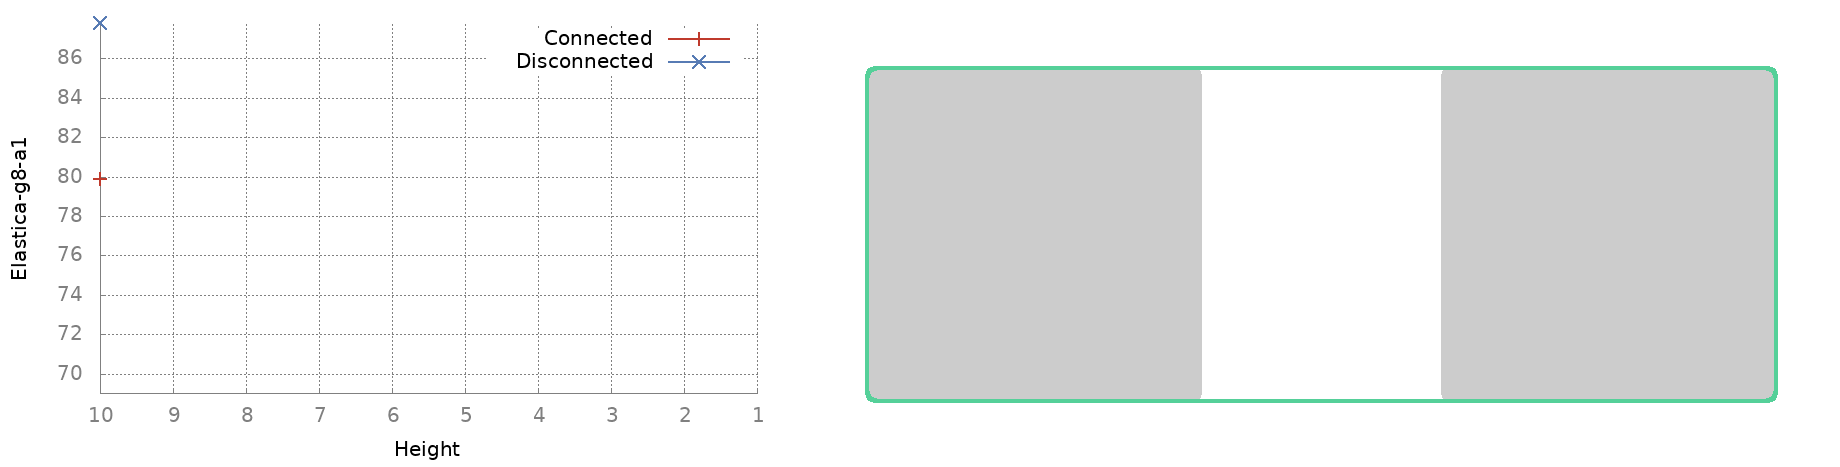
\includegraphics[scale=0.2]{figures/motivation/completion/elastica-g8a1-0.png}
}%
\only<2>{
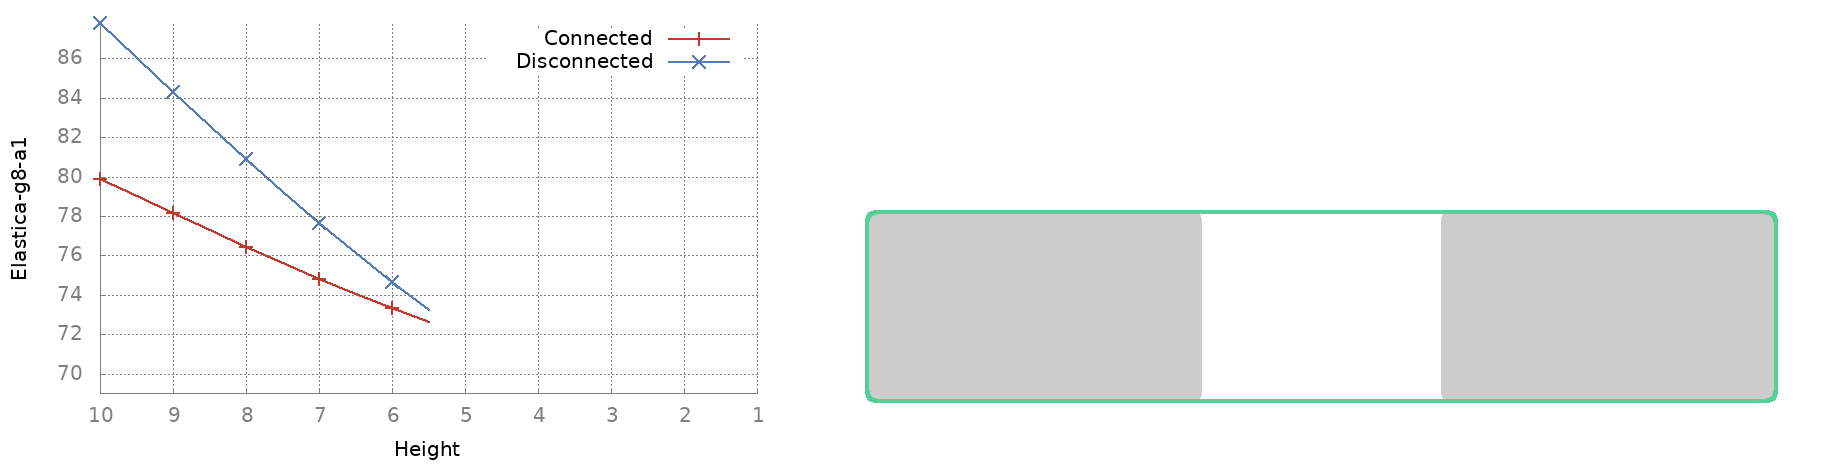
\includegraphics[scale=0.2]{figures/motivation/completion/elastica-g8a1-1.png}
}%
\only<3>{
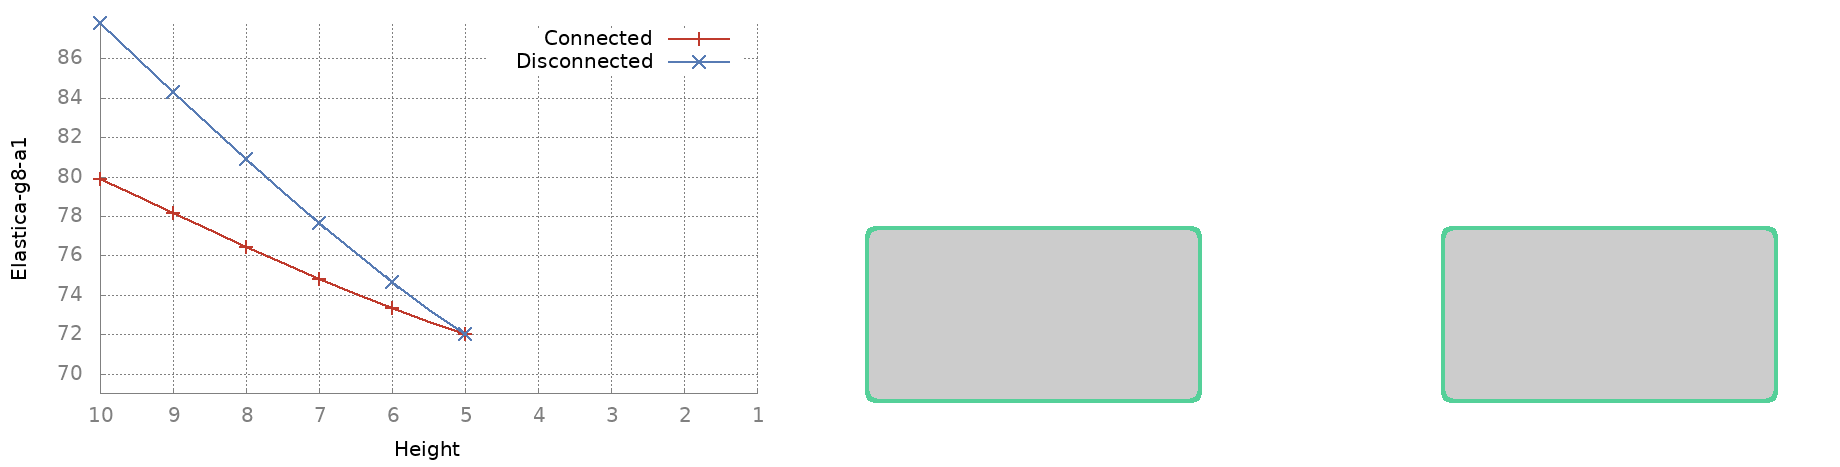
\includegraphics[scale=0.2]{figures/motivation/completion/elastica-g8a1-2.png}
}%
\only<4>{
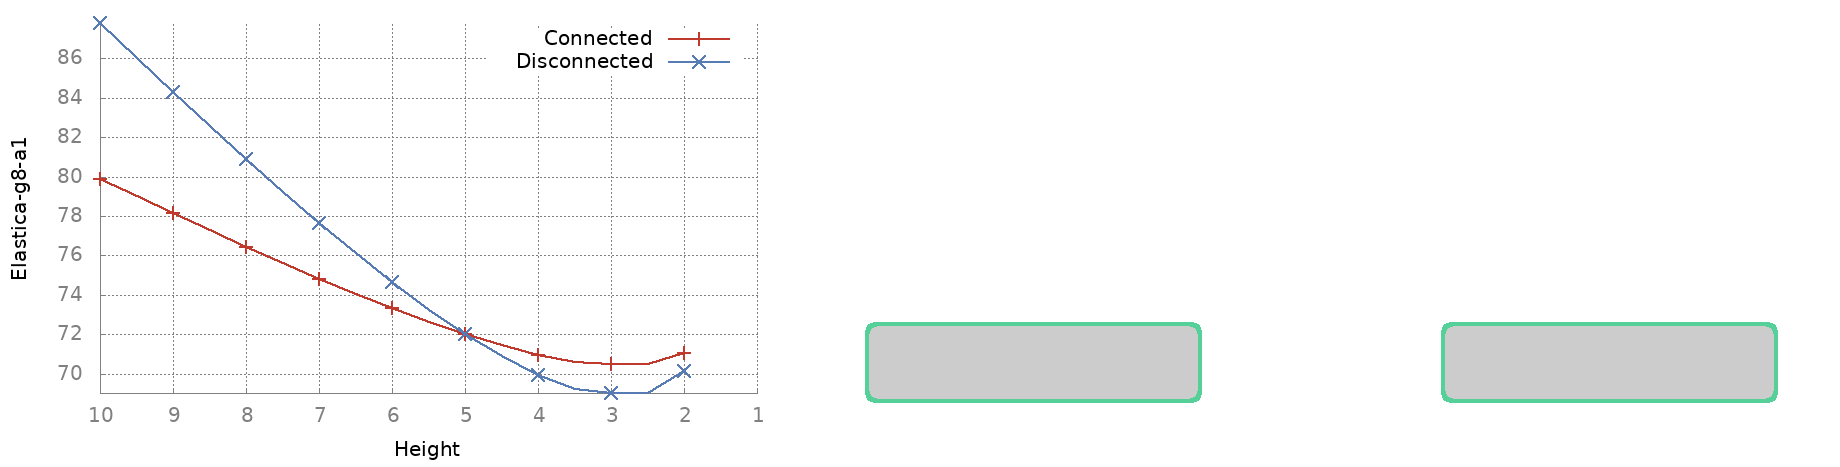
\includegraphics[scale=0.2]{figures/motivation/completion/elastica-g8a1-3.png}
}%
\only<5->{
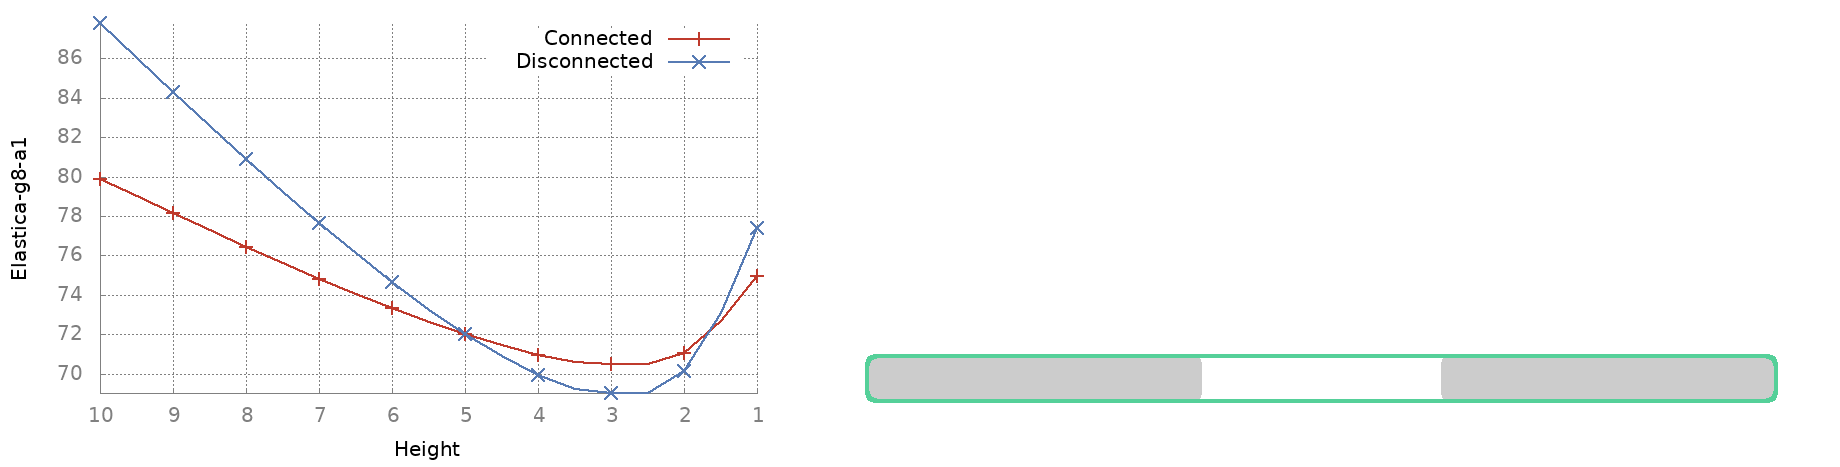
\includegraphics[scale=0.2]{figures/motivation/completion/elastica-g8a1-4.png}
}%
%
\begin{tikzpicture}
    \node at (current page.north east)
        {%
        \begin{tikzpicture}[remember picture, overlay]
		\draw [xshift=0.6cm,yshift=1.2cm,decorate,decoration={brace,amplitude=5pt,mirror,raise=4ex}]
		  (1,0) -- (2.5,0) node[midway,yshift=-3em]{Larger gap};
	  \end{tikzpicture}
	  };%
\end{tikzpicture}
%
\end{minipage}
\begin{minipage}[t][0.45\textheight][t]{\textwidth}
\only<6-10>{
\center
$\min_{ X \subset \Omega } Data(X) + {\color{highlightcolor} \frac{1}{2}} Perimeter(\partial X) + Curvature^2(\partial X).$\\[1em]
}
\only<6>{
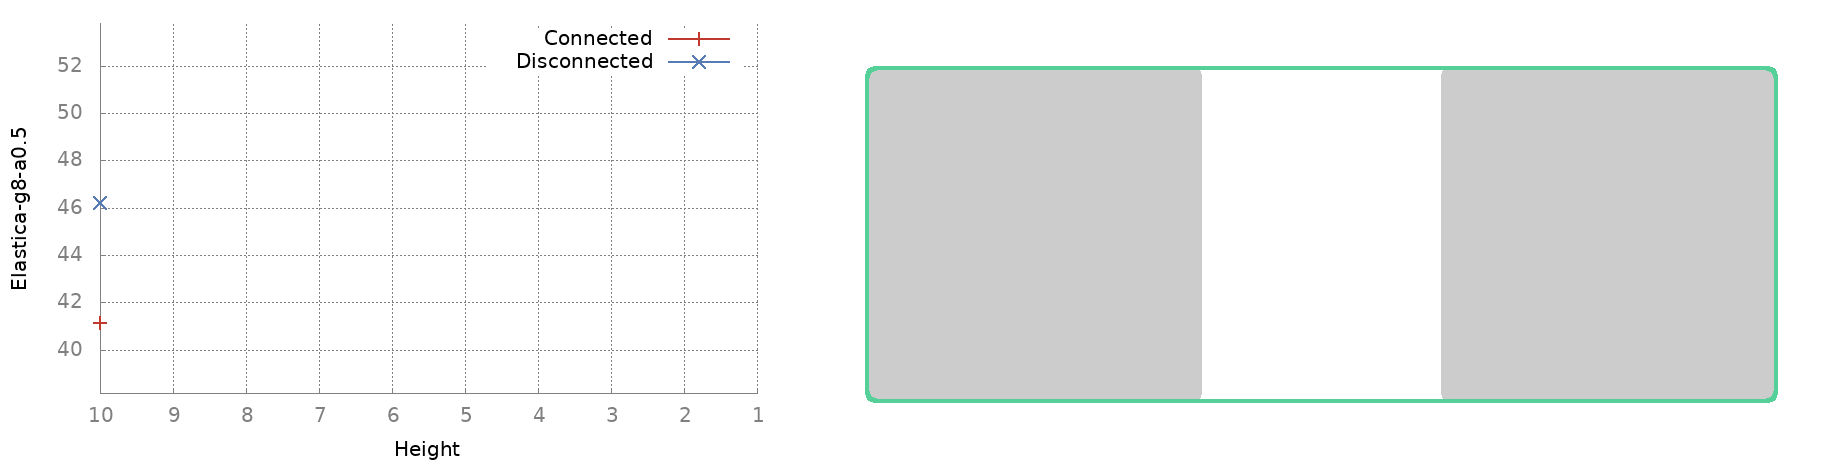
\includegraphics[scale=0.2]{figures/motivation/completion/elastica-g8a05-0.png}
}
\only<7>{
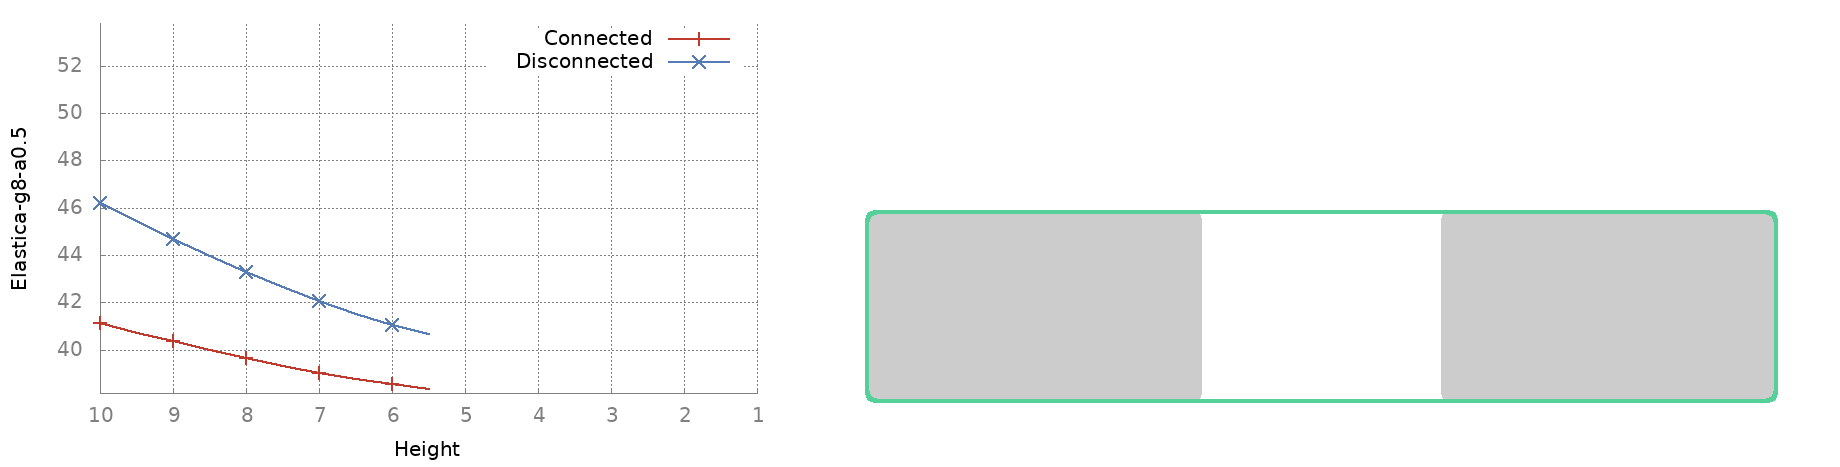
\includegraphics[scale=0.2]{figures/motivation/completion/elastica-g8a05-1.png}
}
\only<8>{
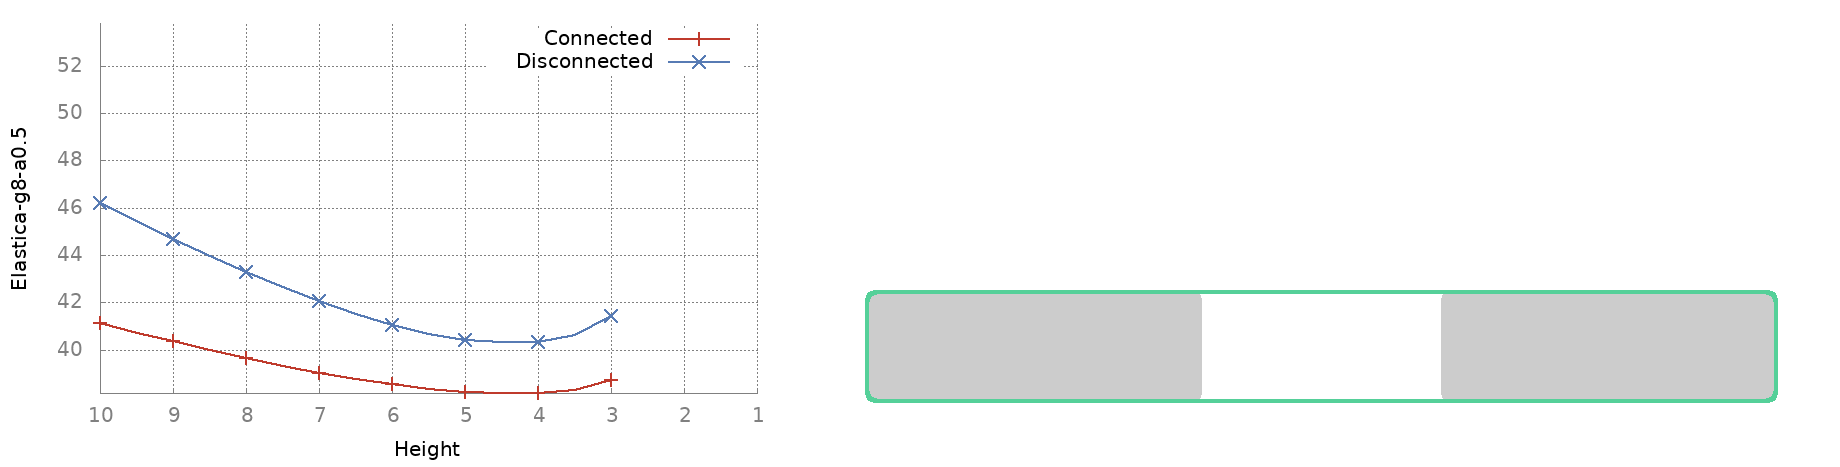
\includegraphics[scale=0.2]{figures/motivation/completion/elastica-g8a05-2.png}
}
\only<9->{
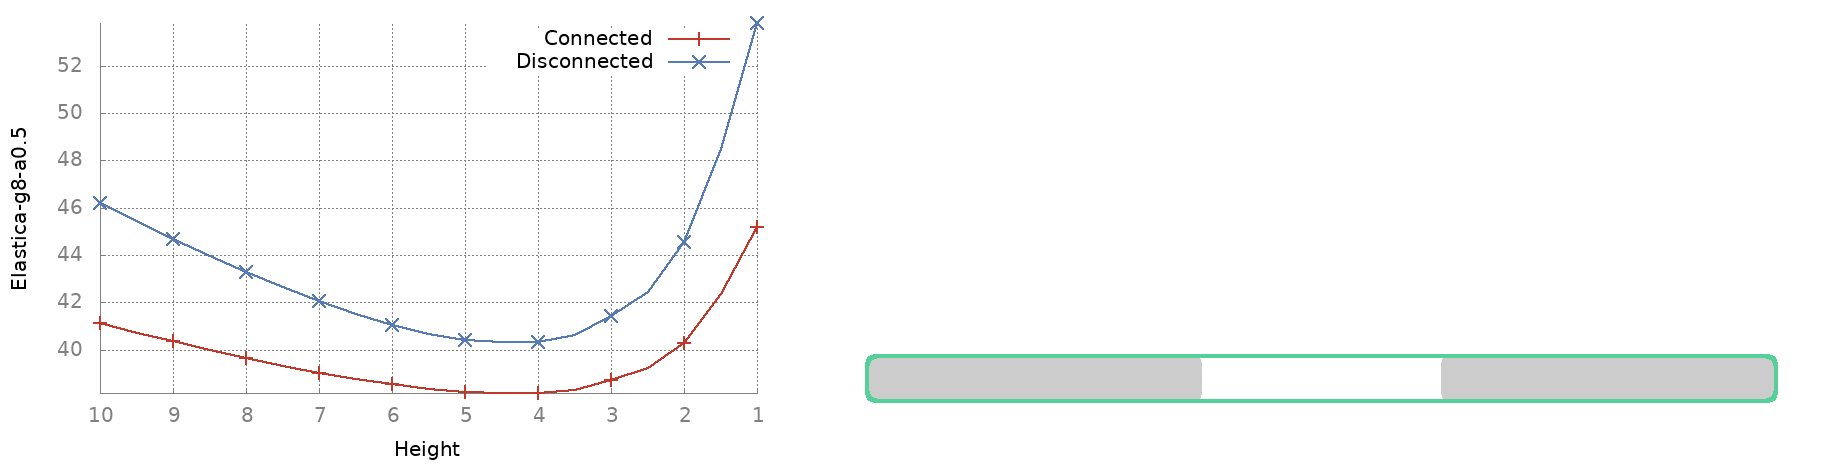
\includegraphics[scale=0.2]{figures/motivation/completion/elastica-g8a05-3.png}
}
\onslide<10>{
	\begin{figure}
	\begin{tikzpicture}[overlay, remember picture] 
	\node at (current page.center) 
	    [
	    anchor=east,
	    xshift=-10mm,
	    yshift=0mm
	    ] 
	{
	
	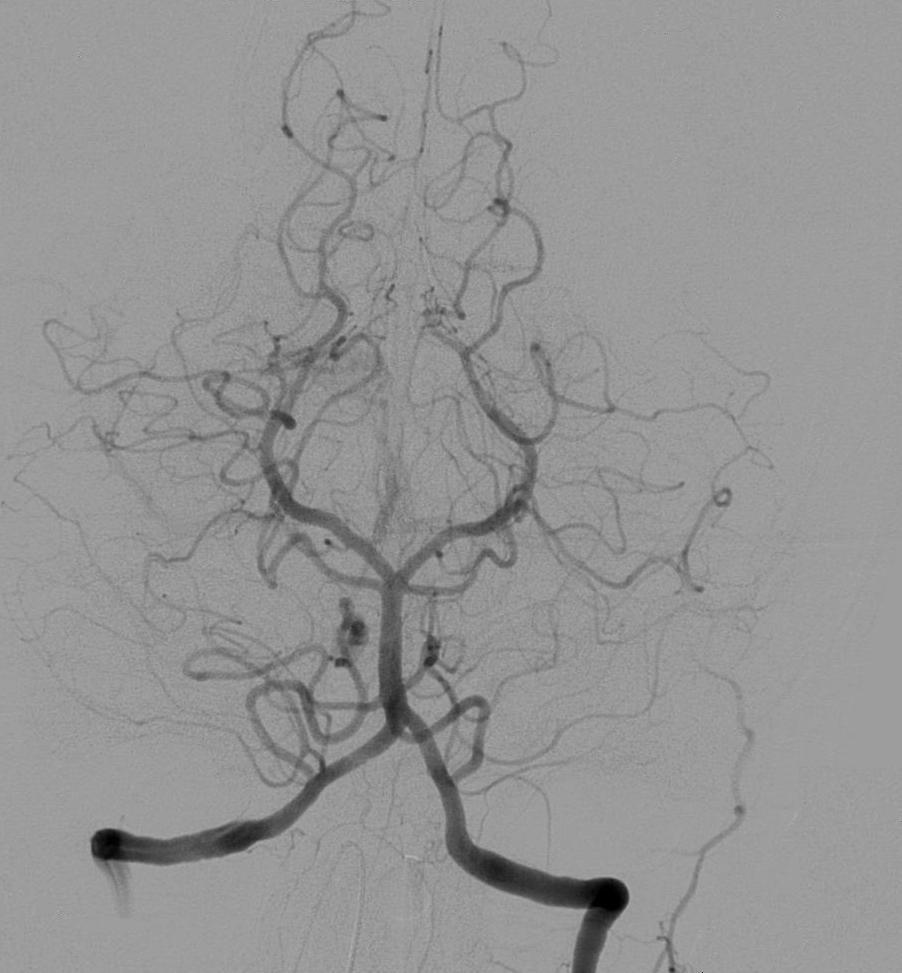
\includegraphics[scale=0.16]{figures/motivation/completion/angiogram.jpg}
		
	};
	\node at (current page.center) 
	    [
	    anchor=west,
	    xshift=-10mm,
	    yshift=0mm
	    ] 
	{
	
	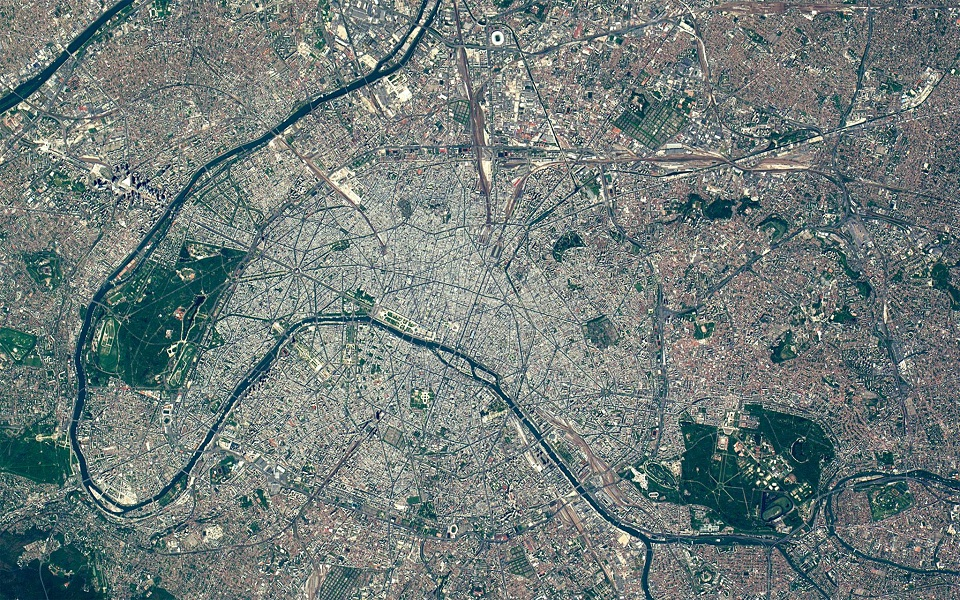
\includegraphics[scale=0.35]{figures/motivation/completion/paris-satellite-road.jpg}
		
	};	
	\end{tikzpicture}	
	\end{figure}	
	}	
\end{minipage}
\end{frame}

\subsection*{Related Works}

\begin{frame}
{Related works}

\begin{itemize}
	\item{Minimize the elastica of level curves~ \mycite{chan02elasticainpainting}.}
	\begin{itemize}
		\item{Numerical instability (4th order Euler-Lagrange equation).}
	\end{itemize}
	\item{T-junctions matching~\mycite{masnou98inpainting}}
	\begin{itemize}
		\item{Limited to polygonal solutions.}
	\end{itemize}
	\item{Linear programming~\mycite{schoenemann09linear}}
	\begin{itemize}
		\item{Prohibitive running times.}
	\end{itemize}
	\item{Triple cliques~\mycite{nieuwenhuis14efficient}}
	\begin{itemize}
		\item{Good precision is conditioned to large neighborhoods ($=$ high running time).}
	\end{itemize}
	\item{Morphological active contour~\mycite{marquez2013morphological}}
	\begin{itemize}
		\item{Related to our implementation of the curve-shortening flow. Data term injection is not simple, though.}
	\end{itemize}	
\end{itemize}
\end{frame}



\section*{Proposed model}
\subsection{Digital estimators \\[1em]Curve-shortening flow \\[1em]Elastica shape optimization \\[1em] Applications in imaging}

\begin{frame}
{Digital set peculiarities}

\textbf{Exact sampling x digitization}

\begin{center}
\begin{tabular}{ccc}
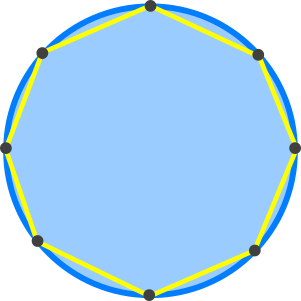
\includegraphics[scale=0.45]{figures/digital-estimators/exact-sampling/sampling-0.png}&
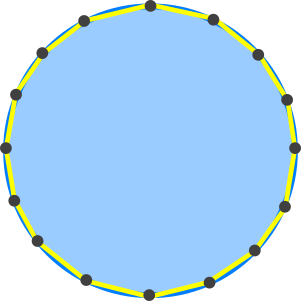
\includegraphics[scale=0.45]{figures/digital-estimators/exact-sampling/sampling-1.png}&
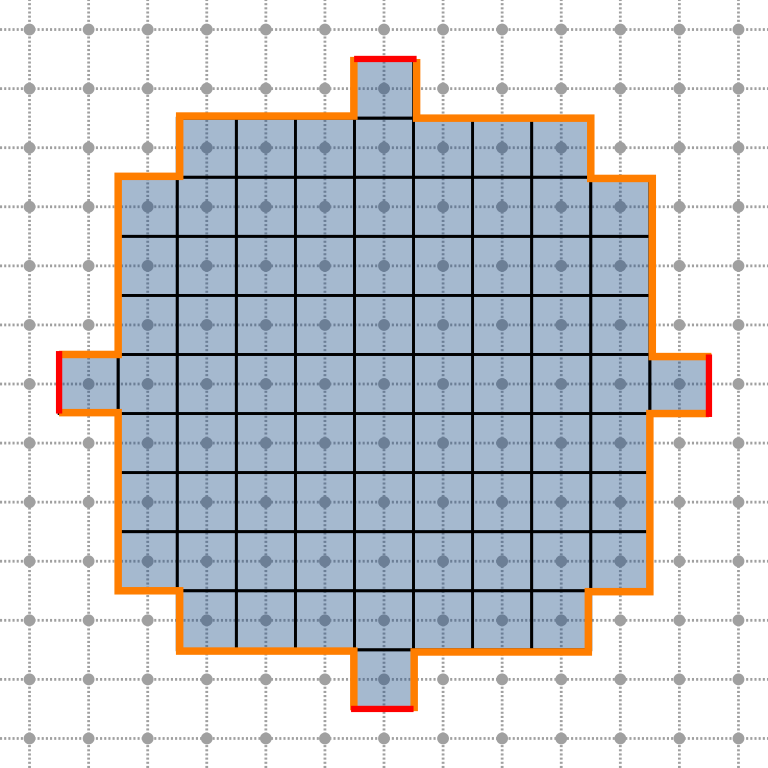
\includegraphics[scale=0.22]{figures/digital-estimators/exact-sampling/digital-ball-perimeter.png}
\end{tabular}
\end{center}

\pause
\textbf{Digitization ambiguity}

\begin{center}
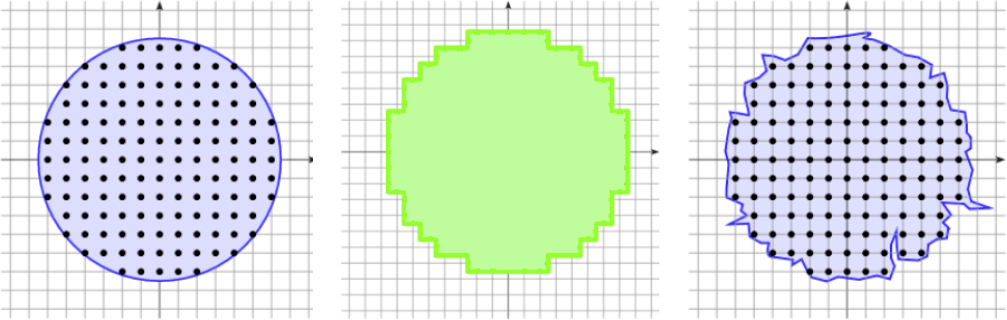
\includegraphics[scale=1]{figures/digital-estimators/exact-sampling/ambiguity.png}
\end{center}

\end{frame}

\begin{frame}
{Multigrid convergent estimators}

\footnotesize

\center
Disk of radius $5 (Area\approx78.54).$ 

\center
\begin{tabular}{ccc}
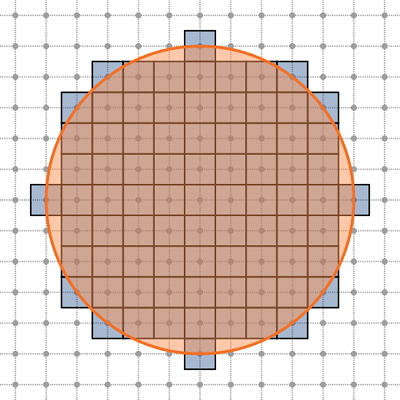
\includegraphics[scale=0.4]{figures/digital-estimators/multigrid/h1.png} &
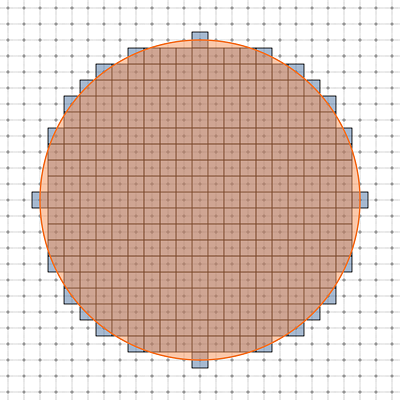
\includegraphics[scale=0.4]{figures/digital-estimators/multigrid/h05.png} &
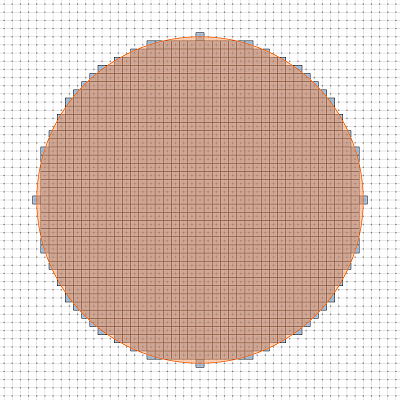
\includegraphics[scale=0.4]{figures/digital-estimators/multigrid/h025.png} \\
$h=1.0,\; \widehat{A}=81.$ & $h=\frac{1}{2},\; \hat{A}=79.25.$ & $h=\frac{1}{4},\; \hat{A}=78.56.$\\[1em]
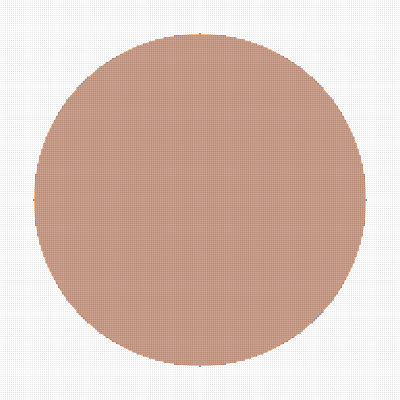
\includegraphics[scale=0.4]{figures/digital-estimators/multigrid/h00625.png} &

\includegraphics[scale=0.4]{figures/digital-estimators/multigrid/h003125.png} &

\includegraphics[scale=0.4]{figures/digital-estimators/multigrid/h003125.png} \\
$h=\frac{1}{16},\; \hat{A}=78.44.$ & $h=\frac{1}{32},\; \hat{A}=78.5.$ & $h=\frac{1}{64},\; \hat{A}=78.53.$
\end{tabular}

\end{frame}

\begin{frame}
	{Digital sets and convergent estimators}	
	{Multigrid convergent estimators}	
%
	\begin{itemize}
		\onslide<1->{\item{Minimum Length Polygon (MLP)~\mycite{sloboda98approximation}}
		\begin{itemize}
			\item{Proved multigrid convergent for piecewise $3$-smooth convex shapes.}
		\end{itemize}}
		\onslide<3->{\vspace{2em}
		\item{Integral Invariant (II)~\mycite{coeurjolly13integral}}
		\begin{itemize}
			\item{Proved multigrid convergent for $C^2$ convex shapes with bounded curvature.}
		\end{itemize}}		
	\end{itemize}
	
	\onslide<2>{
	\begin{figure}
	\begin{tikzpicture}[overlay, remember picture] 
	\node at (current page.center) 
	    [
	    anchor=center,
	    xshift=0mm,
	    yshift=0mm
	    ] 
	{
	
	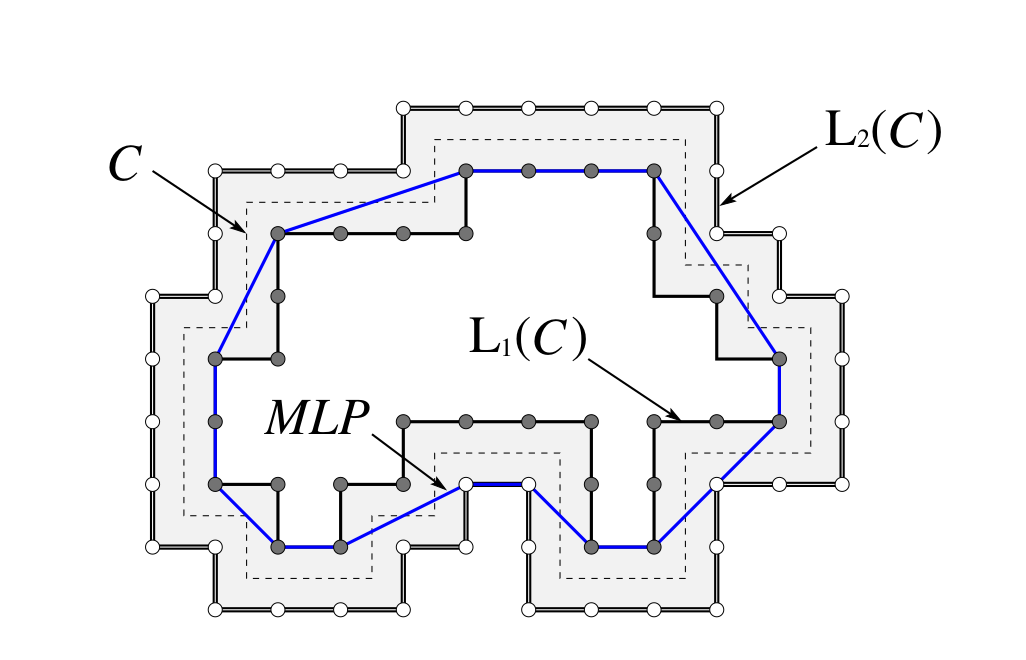
\includegraphics[scale=1.0]{figures/digital-estimators/mlp.png}
		
	};
	\end{tikzpicture}	
	\end{figure}	
	}
	
	\onslide<4->{
	\begin{figure}
	\begin{tikzpicture}[overlay, remember picture] 
	\node at (current page.center) 
	    [
	    anchor=center,
	    xshift=0mm,
	    yshift=0mm
	    ] 
	{
	\only<4>{
	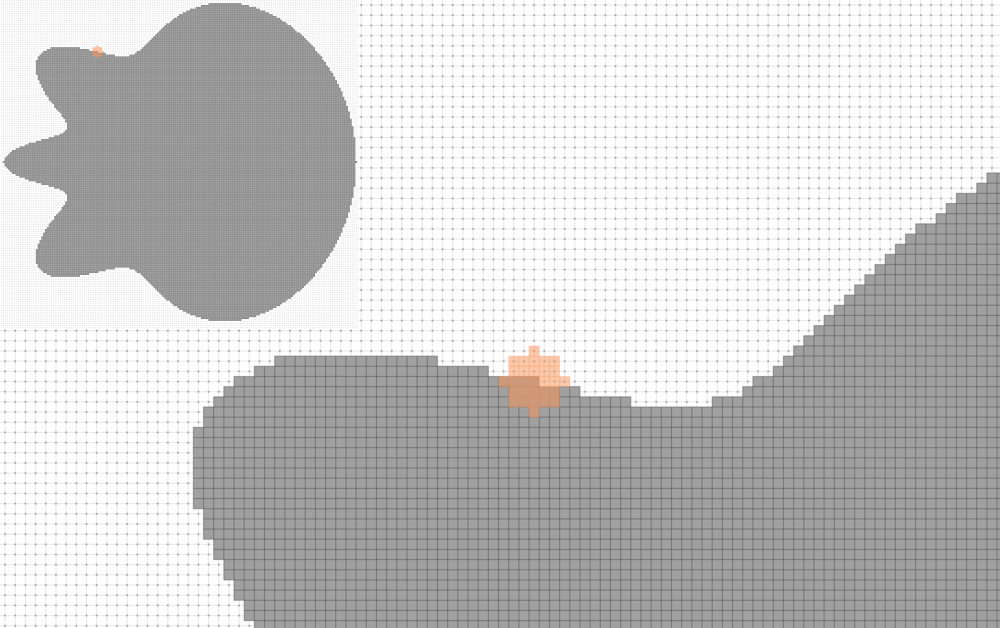
\includegraphics[scale=0.5]{figures/digital-estimators/ii/zoom/fr3-zoom.png}}%
	\only<5>{
	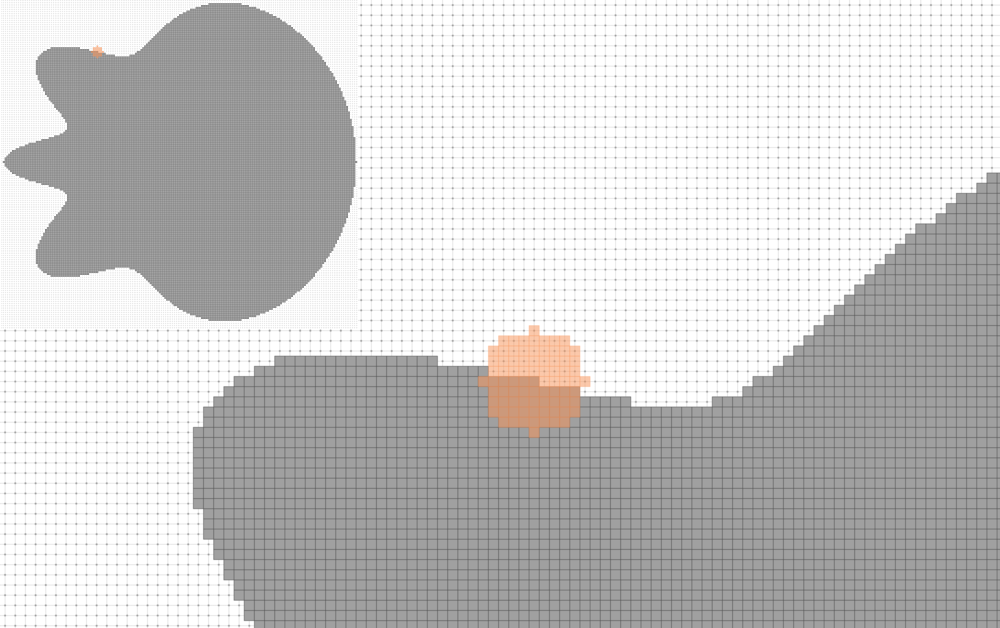
\includegraphics[scale=0.5]{figures/digital-estimators/ii/zoom/fr5-zoom.png}}%
		
	};
	\end{tikzpicture}	
	\end{figure}	
	}	

	\vspace{1.5em}

	\onslide<4->{
	\begin{align*}
		\hat{\kappa}(p) = \frac{3}{r^3}\left( \frac{\pi r^2}{2} - | B_r(p) \cap X | \right )
	\end{align*}}		
	
\end{frame}

\begin{frame}
	{Digital sets and convergent estimators}	
	{Conclusion}	

	\begin{itemize}
		\item{Digital sets are ambiguous and are constrained to the digital grid.}\\[1em]
		\item{The multigrid convergence is an adapted definition of convergence for geometric estimation on digital sets.}\\[2em]\pause
		\item[]{\textbf{Can we construct optimization models using multigrid convergent estimators?}}
	\end{itemize}

\end{frame}
\subsection*{Curve-shortening flow}

\begin{frame}
{Model workflow}

\only<1>{
	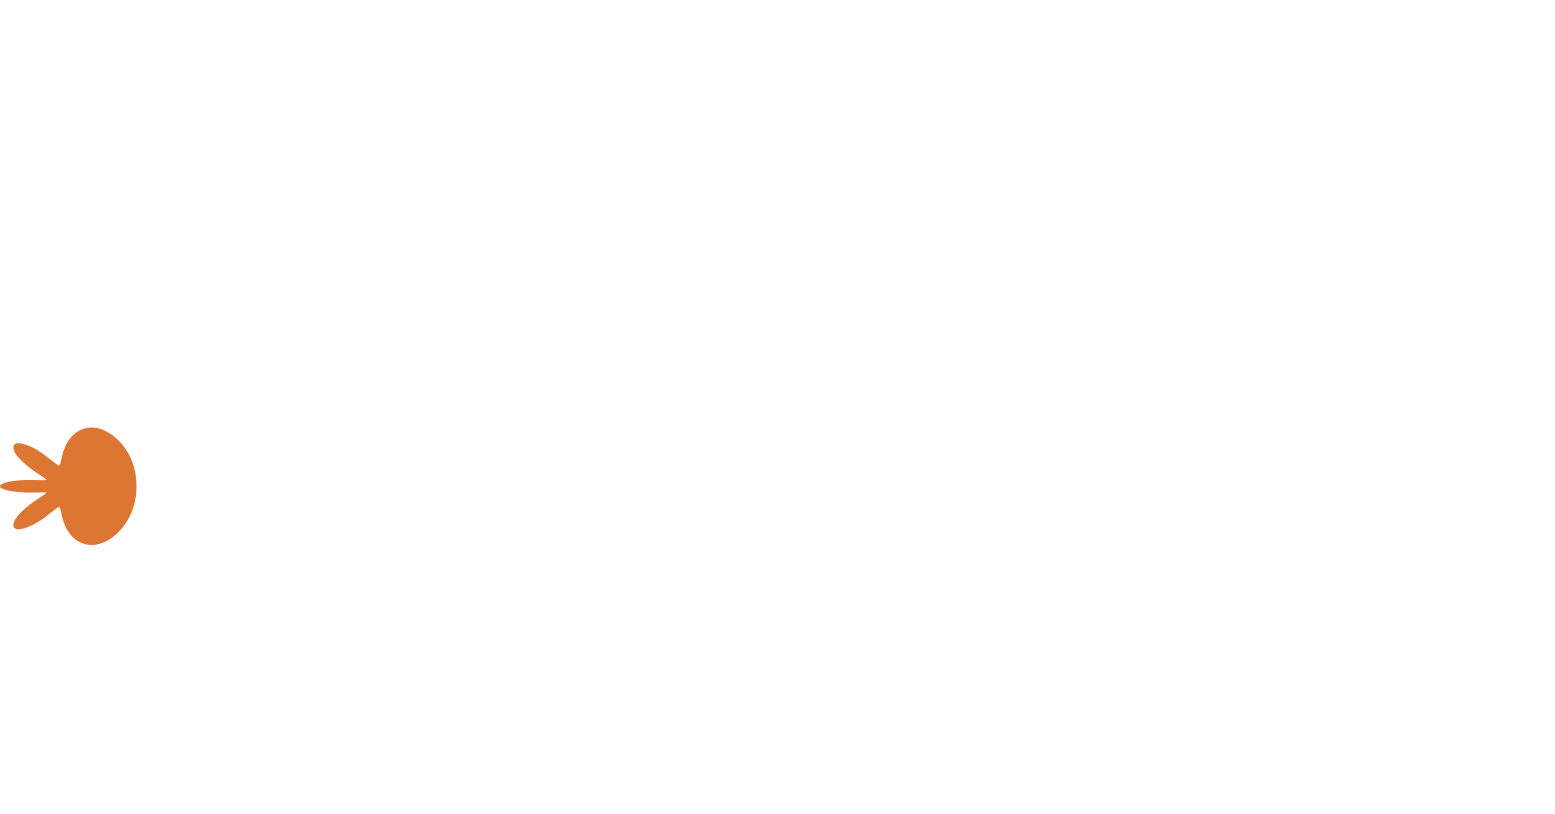
\includegraphics[scale=0.36]{figures/model-workflow/workflow-1.png}}
\only<2>{
	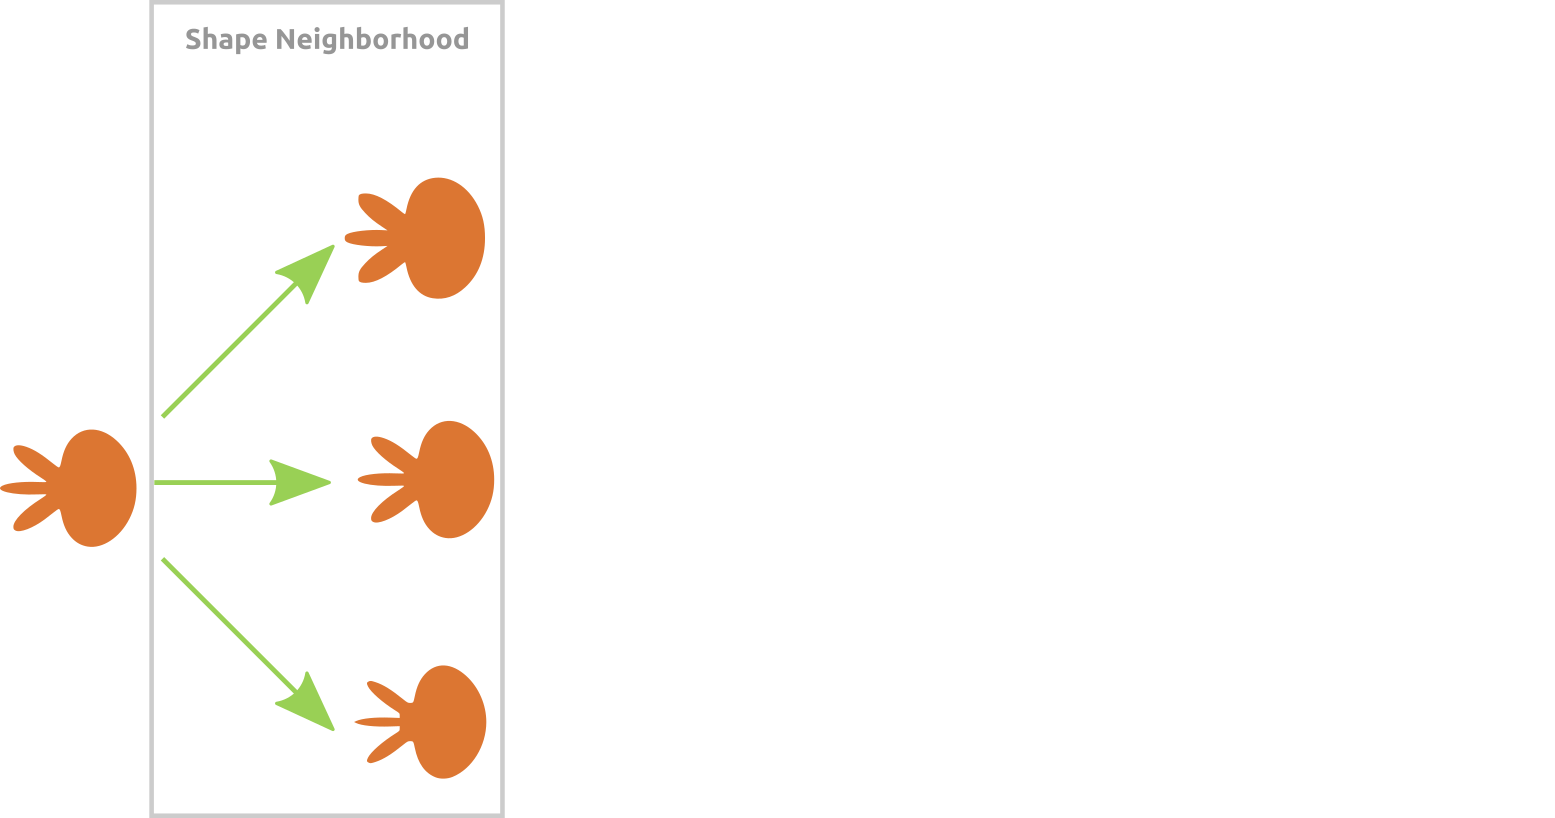
\includegraphics[scale=0.36]{figures/model-workflow/workflow-2.png}}	
\only<3>{
	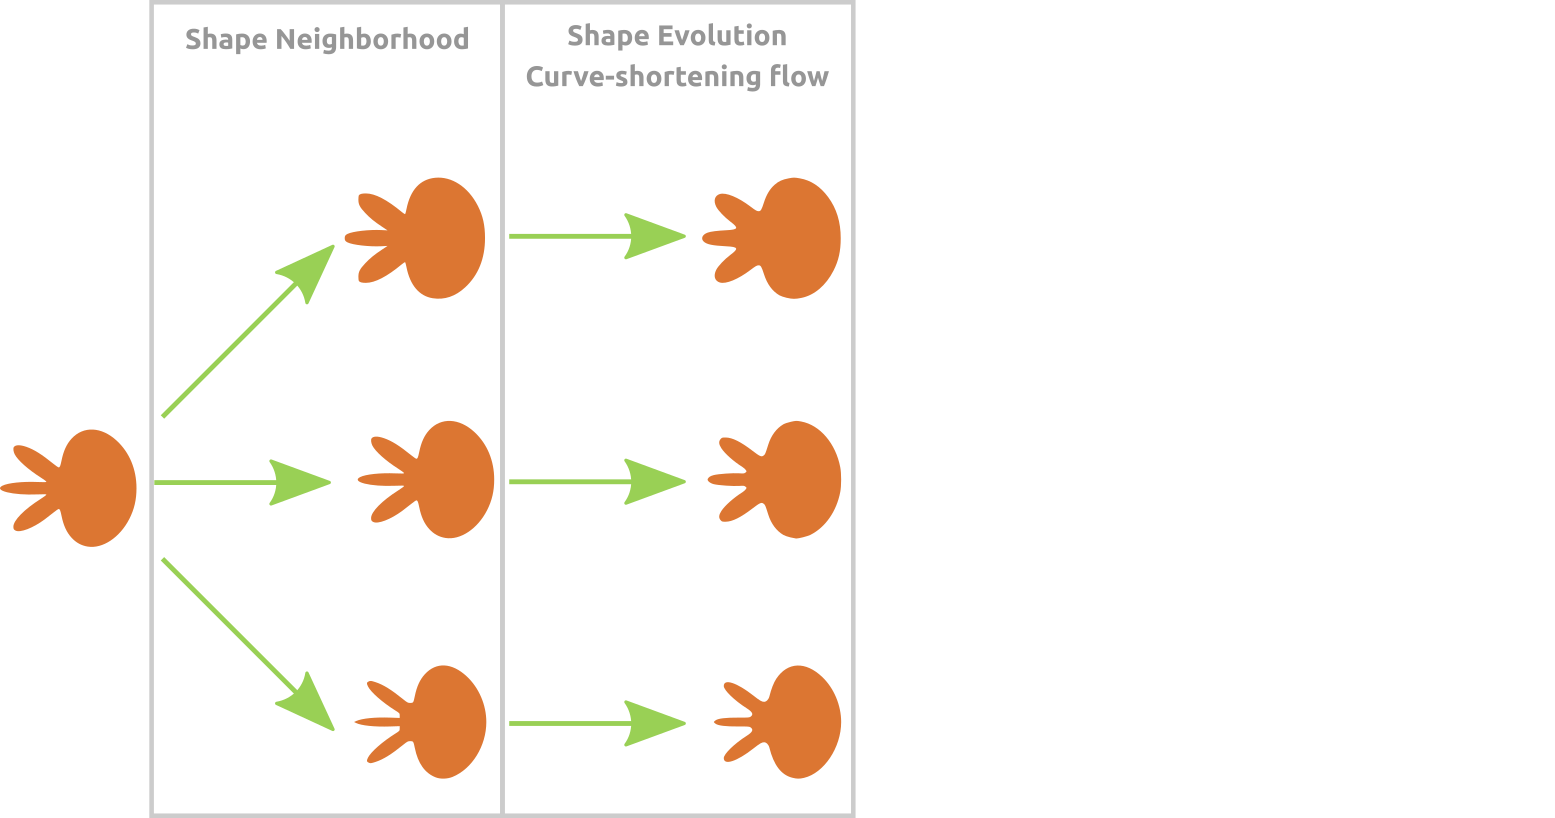
\includegraphics[scale=0.36]{figures/model-workflow/workflow-3.png}}	
\only<4>{
	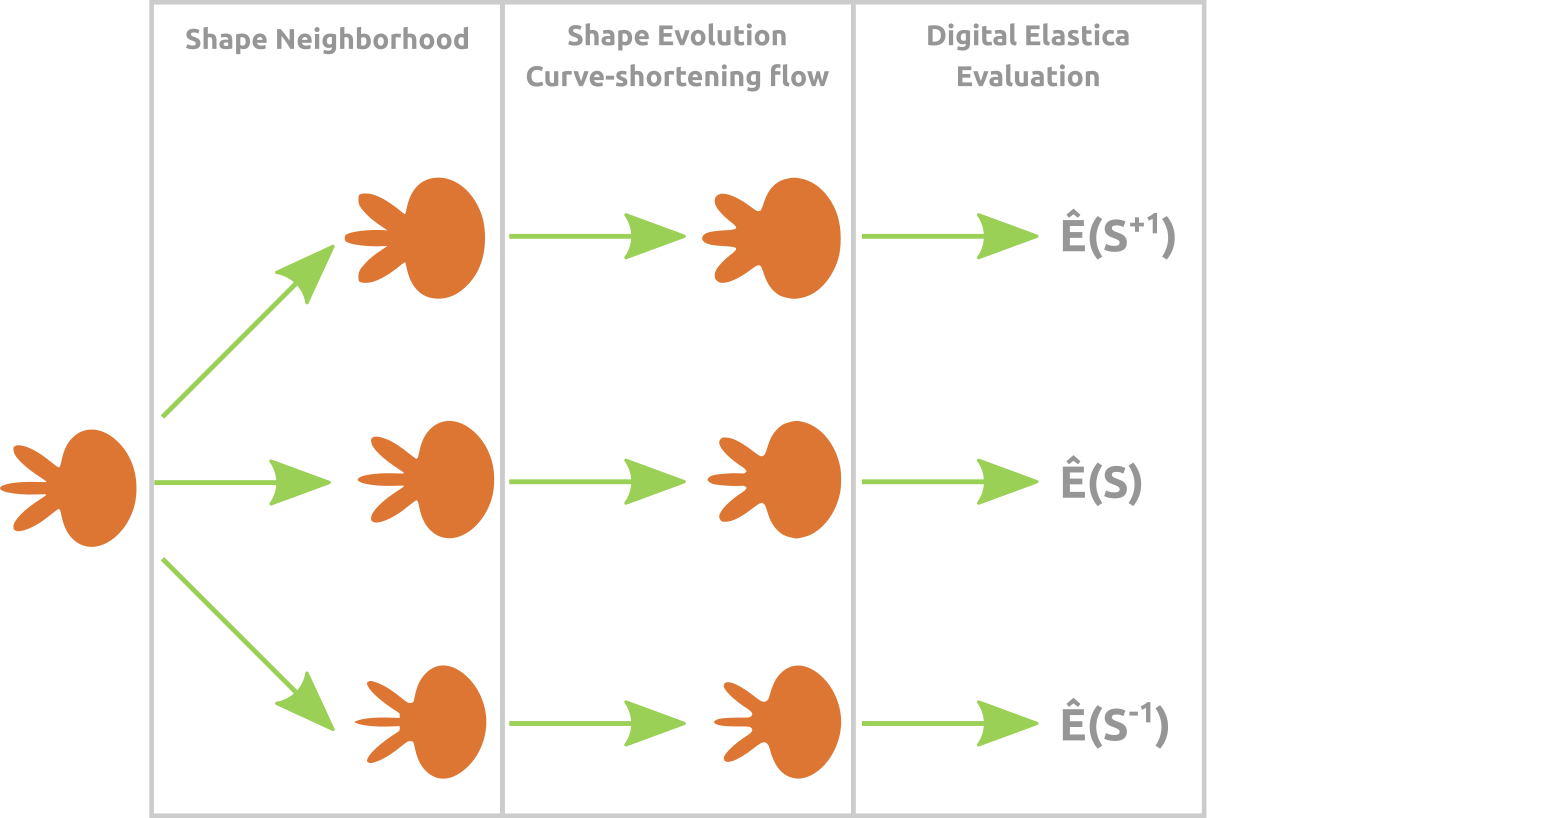
\includegraphics[scale=0.36]{figures/model-workflow/workflow-4.png}}	
\only<5>{
	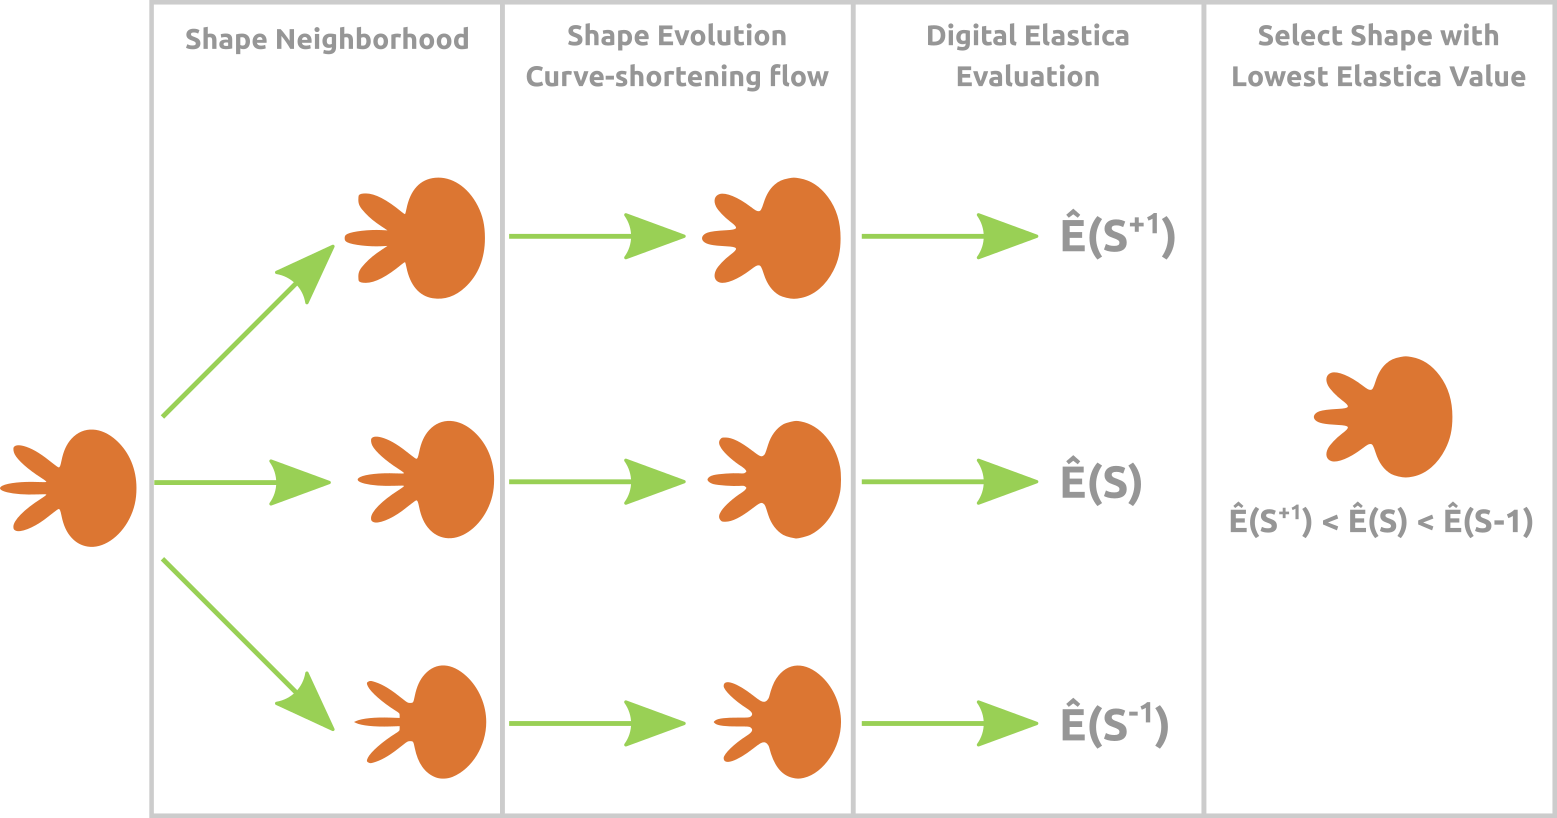
\includegraphics[scale=0.36]{figures/model-workflow/workflow-5.png}}	
\only<6>{
	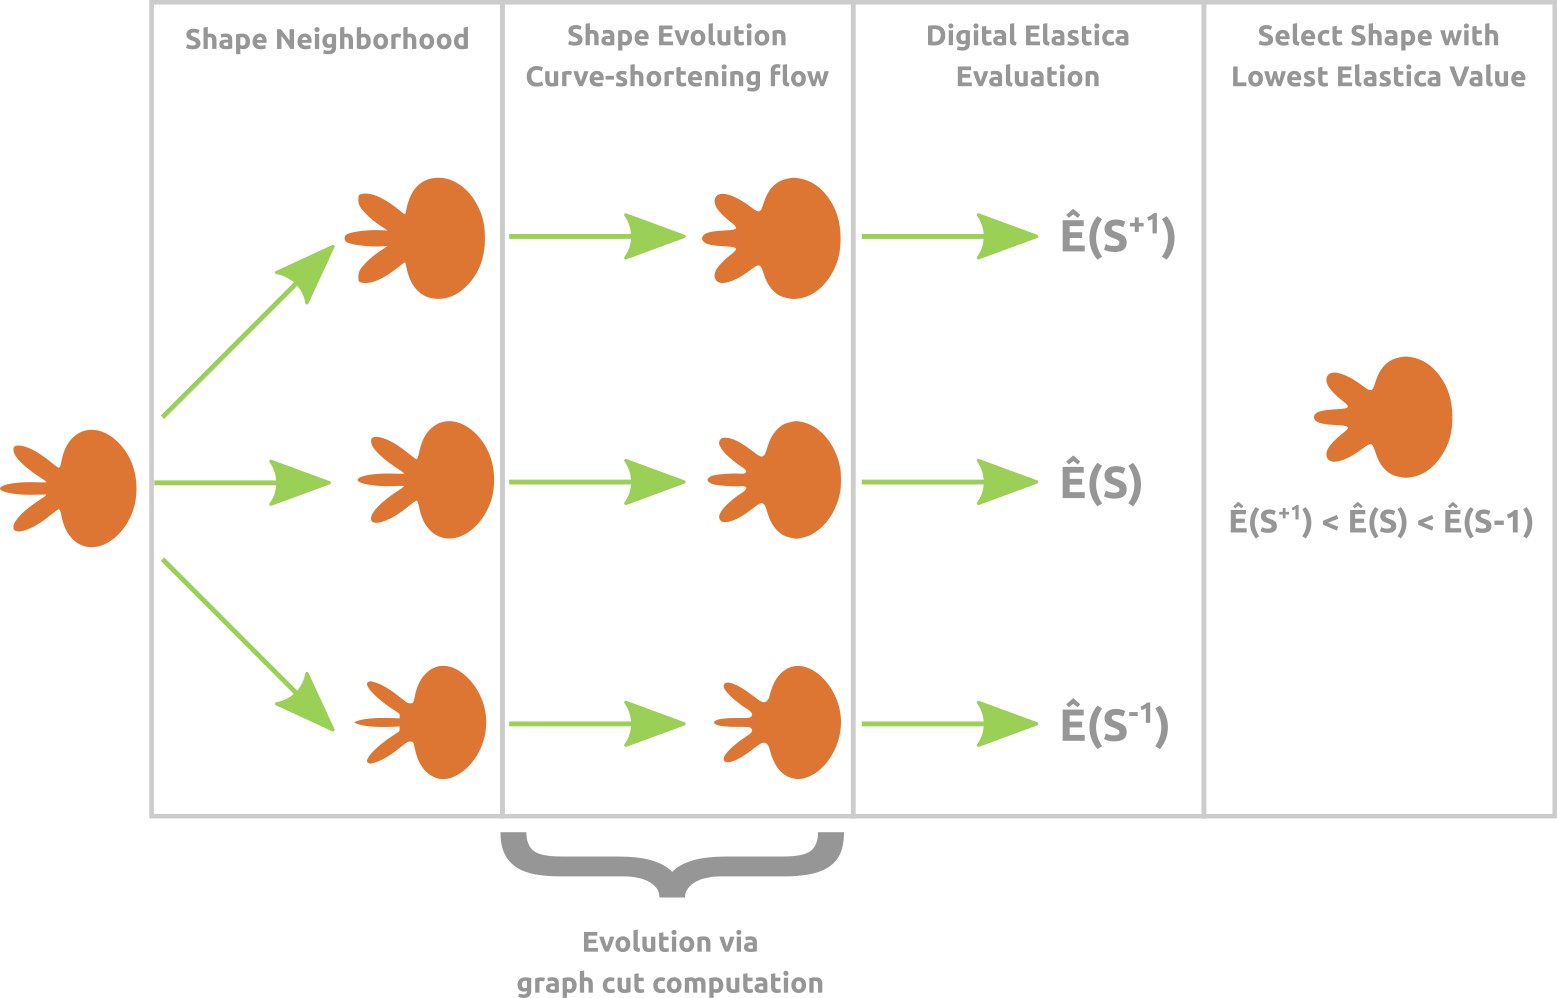
\includegraphics[scale=0.36]{figures/model-workflow/workflow-6.png}}	
\only<7>{
	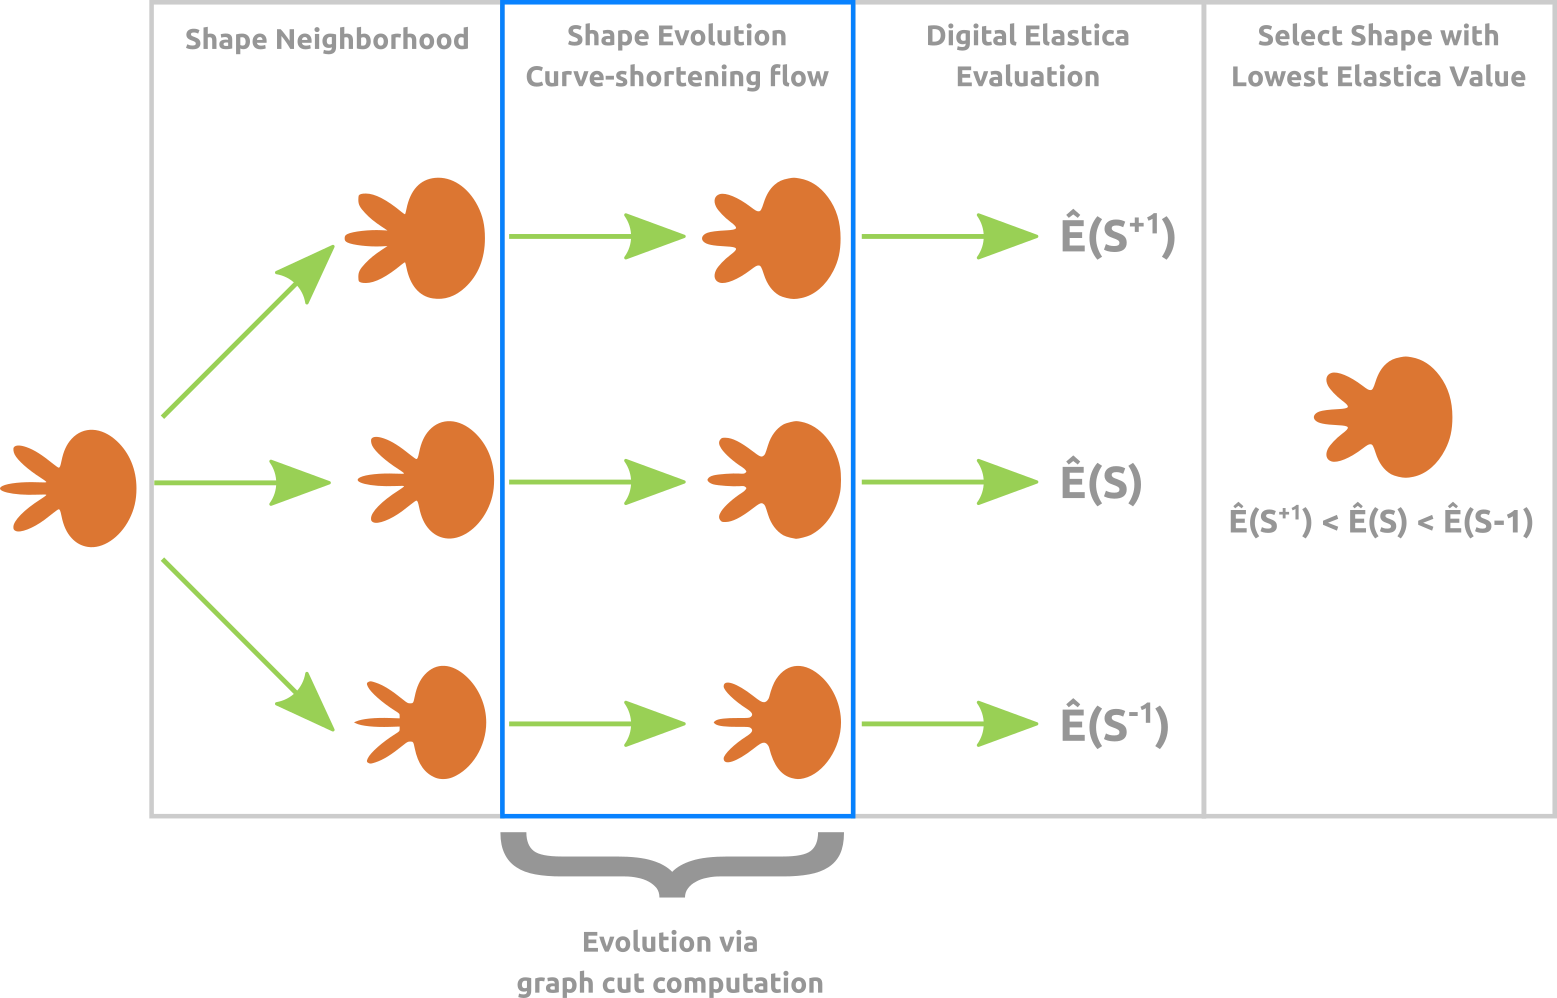
\includegraphics[scale=0.36]{figures/model-workflow/workflow-curve-shortening-flow.png}}	

\end{frame}

\begin{frame}
{Curve-shortening flow}
\begin{minipage}{0.5\textwidth}
\center
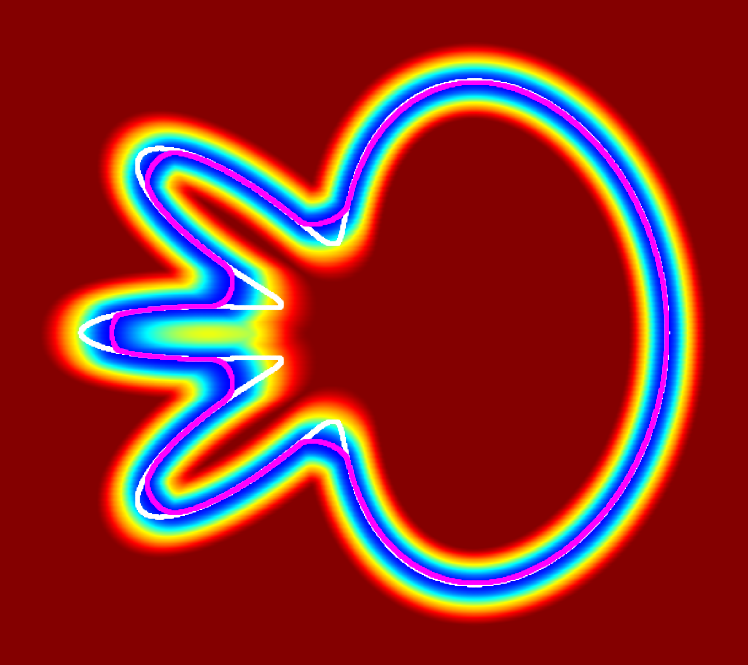
\includegraphics[scale=0.2]{figures/curve-shortening-flow/balance-coefficient-zero-level-set.png}
\end{minipage}
\begin{minipage}{0.49\textwidth}
\footnotesize
\begin{itemize}
\item{Balance coefficient}
\begin{align*}
u_r(D,p) &= \left( \frac{\pi r^2}{2} - |B_r(p) \cap D| \right)^2
\end{align*}
\item{White contour: contour of the shape}
\item{Pink contour: $\epsilon$-level set of the balance coefficient}
\end{itemize}
\end{minipage}
\end{frame}


\begin{frame}
{Curve-shortening flow}

\begin{minipage}{0.3\textwidth}
\only<1>{
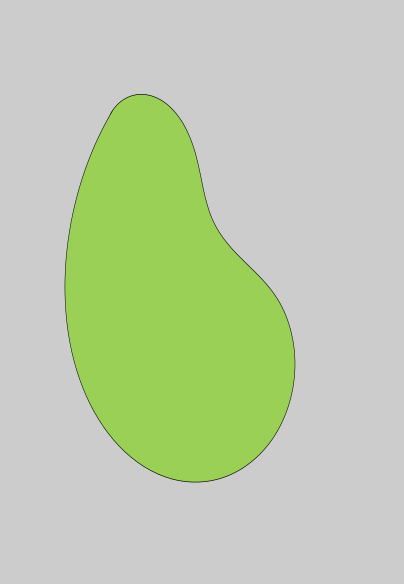
\includegraphics[scale=0.5]{figures/curve-shortening-flow/graph-model-1.png}}%
\only<2-3>{
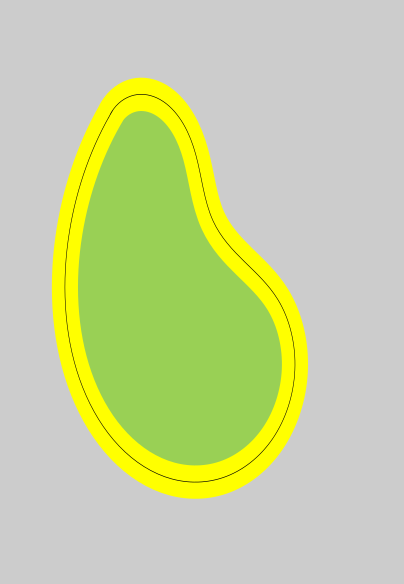
\includegraphics[scale=0.5]{figures/curve-shortening-flow/graph-model-2.png}}%
\only<4->{
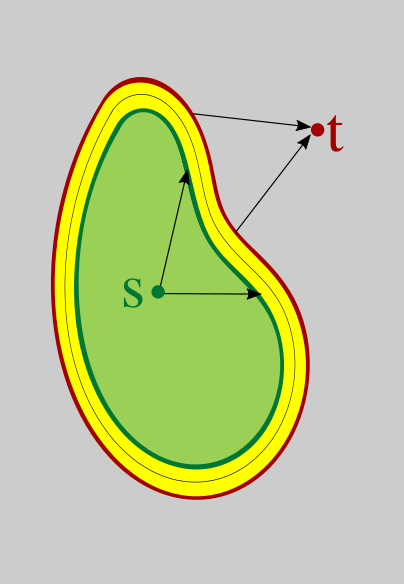
\includegraphics[scale=0.5]{figures/curve-shortening-flow/graph-model-3.png}}%
\end{minipage}
%
%
\begin{minipage}{0.69\textwidth}
\footnotesize
\begin{itemize}
\itemsep0em
\onslide<2->{\item{Optimization band
\begin{align*}
%\only<2>{O_n(D) :=& \{ p \in D \; | \; -n \leq d_D(p) \leq n \} \\}
\only<2->{O(D) :=& \{ p \in D \; | \; -n \leq d_D(p) \leq n \} \\}
\onslide<3->{F(D) :=& D \setminus O(D)}
\end{align*}}\vspace{-1em}}
\onslide<4->{\item{Graph $\mathcal{G}_D(\mathcal{V},\mathcal{E},c)$
\begin{align*}
\mathcal{V} &= \{ v_p \; | \; p \in O(D) \} \cup \{s,t\} \\
\highlight{6}{4,5,7-}{\mathcal{E}} &= \highlight{6}{4,5,7-}{\{ \{v_p,v_q\} \; | \; p,q \in O(D) \text{ and } q \in \mathcal{N}_4(p) \}} \cup \highlight{5}{4,6-}{\mathcal{E}_{st}} \\
\highlight{5}{4,6-}{\mathcal{E}_{st}} &= \highlight{5}{4,6-}{\{ (s,v_p), (v_p,t) \; | \; p \in O(D) \}}
\end{align*}}\vspace{-1em}}
\onslide<7->{\item{Edge's weight
\begin{center}
\begin{tabular}{|c|c|}
\hline
\textbf{edge} $e$ & $\mathbf{c(e)}$\\
\hline
$\{v_p, v_q\}$ & $ \frac{1}{2}\left( u_r(D,p) + u_r(D,q)\right) $\\
\hline
$(s,v_p)$ & $M$\\
\hline
$(v_p, t)$ & $M$\\
\hline
\end{tabular}
\end{center}
}}
\onslide<8->{\item{Digital shape update
\begin{align*}
D^{(k+1)} &= F(D^{(k)}) + S^{(k)}
\end{align*}}}
\end{itemize}
\end{minipage}
\end{frame}
%
%
%
\begin{frame}
{Curve-shortening flow}

\begin{center}

\begin{tabular}{cc}
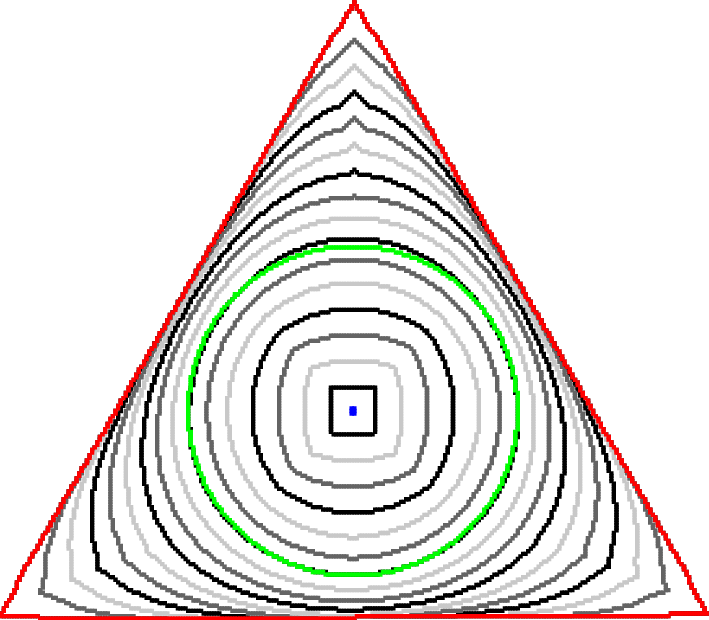
\includegraphics[scale=0.1]{figures/curve-shortening-flow/no-neighborhood-flow-always-evolve/0.015625/triangle.png}\hspace{3em} &
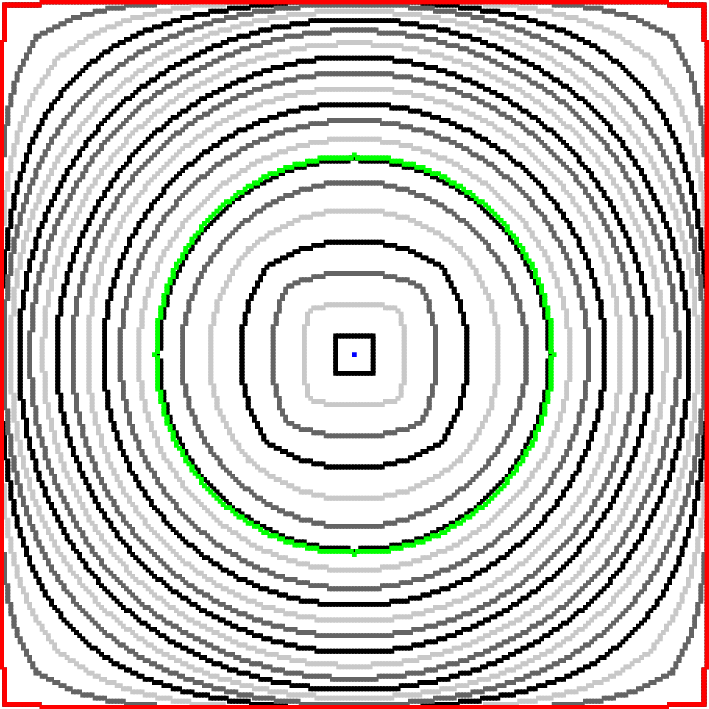
\includegraphics[scale=0.08]{figures/curve-shortening-flow/no-neighborhood-flow-always-evolve/0.015625/square.png}\\[1em]
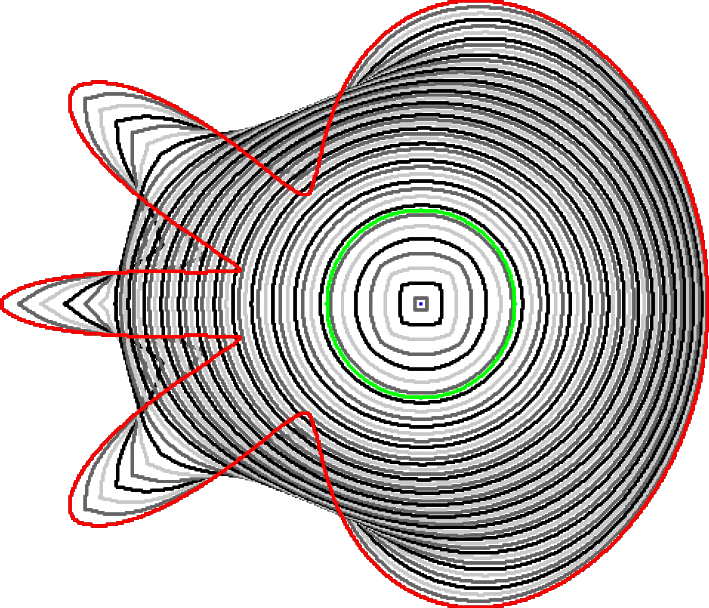
\includegraphics[scale=0.12]{figures/curve-shortening-flow/no-neighborhood-flow-always-evolve/0.015625/flower.png}\hspace{3em} &
\includegraphics[scale=0.12]{figures/curve-shortening-flow/no-neighborhood-flow-always-evolve/0.015625/bean.png}
\end{tabular}
\end{center}

\end{frame}
\begin{frame}
{Elastica shape optimization}

\center

\begin{tabular}{cc}
\includegraphics[scale=0.12]{figures/elastica-minimization/with-neighborhood-flow/radius_16/triangle.png}\hspace{3em} &
\includegraphics[scale=0.12]{figures/elastica-minimization/with-neighborhood-flow/radius_16/square.png}\\[2em]
\includegraphics[scale=0.12]{figures/elastica-minimization/with-neighborhood-flow/radius_16/flower.png}\hspace{3em} &
\includegraphics[scale=0.12]{figures/elastica-minimization/with-neighborhood-flow/radius_16/bean.png}
\end{tabular}

\end{frame}

\begin{frame}
{Elastica shape optimization}

\begin{minipage}{0.25\textwidth}
\center
\includegraphics[scale=0.06]{figures/elastica-minimization/with-neighborhood-flow/radius_16/triangle.png}\\[1em]
\includegraphics[scale=0.06]{figures/elastica-minimization/with-neighborhood-flow/radius_16/square.png}\\[1em]
\includegraphics[scale=0.06]{figures/elastica-minimization/with-neighborhood-flow/radius_16/flower.png}\\[1em]
\includegraphics[scale=0.06]{figures/elastica-minimization/with-neighborhood-flow/radius_16/bean.png}
\end{minipage}%
%
%
\begin{minipage}{0.74\textwidth}
\center
\includegraphics[scale=0.18]{figures/elastica-minimization/with-neighborhood-flow/plots/elastica.png}\\
\includegraphics[scale=0.18]{figures/elastica-minimization/with-neighborhood-flow/plots/bars.png}
\end{minipage}
\end{frame}

\subsection*{Applications in imaging}

\begin{frame}
{Applications in imaging}

\includegraphics[scale=0.36]{figures/model-workflow/workflow-8.png}

\end{frame}

\begin{frame}
{Applications in imaging}

\begin{minipage}[t][0.45\textheight][t]{\textwidth}
\center
\includegraphics[scale=0.22]{figures/applications-imaging/contour-correction/kite/gc-seg.png}

Classical graph cut
\end{minipage}
\begin{minipage}[t][0.55\textheight][t]{0.5\textwidth}
\center
\includegraphics[scale=0.22]{figures/applications-imaging/contour-correction/kite/corrected-seg-without-data.png}

Our model without data
\end{minipage}%
\begin{minipage}[t][0.55\textheight][t]{0.5\textwidth}
\center
\includegraphics[scale=0.22]{figures/applications-imaging/contour-correction/kite/corrected-seg-with-data.png}

Our model with data
\end{minipage}%

\end{frame}

\begin{frame}
{Applications in imaging}

\begin{minipage}[t][0.45\textheight][t]{\textwidth}
\center
\includegraphics[scale=0.25]{figures/applications-imaging/contour-correction/moto/gc-seg.png}

Classical graph cut
\end{minipage}
\begin{minipage}[t][0.55\textheight][t]{0.5\textwidth}
\center
\includegraphics[scale=0.25]{figures/applications-imaging/contour-correction/moto/corrected-seg-without-data.png}

Our model without data
\end{minipage}%
\begin{minipage}[t][0.55\textheight][t]{0.5\textwidth}
\center
\includegraphics[scale=0.25]{figures/applications-imaging/contour-correction/moto/corrected-seg-with-data.png}

Our model with data
\end{minipage}%

\end{frame}

\begin{frame}
{Applications in imaging}

\begin{minipage}[t][0.45\textheight][t]{\textwidth}
\center
\includegraphics[scale=0.22]{figures/applications-imaging/contour-correction/cup/gc-seg.png}

Classical graph cut
\end{minipage}
\begin{minipage}[t][0.55\textheight][t]{0.5\textwidth}
\center
\includegraphics[scale=0.22]{figures/applications-imaging/contour-correction/cup/corrected-seg-without-data.png}

Our model without data
\end{minipage}%
\begin{minipage}[t][0.55\textheight][t]{0.5\textwidth}
\center
\includegraphics[scale=0.22]{figures/applications-imaging/contour-correction/cup/corrected-seg-with-data.png}

Our model with data
\end{minipage}%

\end{frame}





\section{Conclusion}

\begin{frame}
{Conclusion}
{Summary of models}

\onslide<1->{
\begin{table}[H]
\footnotesize
\centering
\begin{tabular}{r|ccccc}
Model & Implementation & RT & Free & Constrained & Image\\
\hline
LocalSearch (LS) & medium & slow & yes(opt) & yes & no \\
FlipFlow (FF) & hard & acceptable & yes & no & yes \\
BalanceFlow (BF) & medium & acceptable & yes & no & yes \\
GraphFlow (GF) & easy & fast & yes(opt) & yes & yes
\end{tabular}
\caption{\textbf{Models summary.} The qualitative attributes are relative, e.g., the GraphFlow presents the lowest running time while LocalSearch presents the highest.}
\end{table}}

\onslide<2->{
\begin{figure}
\center
\captionsetup{type=table}
\footnotesize
\begin{tabular}{|l|c|c|c|c|c|}
\hline
& Pixels & LocalSearch & FlipFlow & BalanceFlow & GraphFlow \\
\hline
Triangle & 8315 & 4.8s/it & 0.4s/it & 0.38s/it & 0.14s/it\\
Square & 12769 & 2s/it & 0.51s/it & 0.47s/it & 0.12s/it\\
Ellipse  & 10038 & 3.1s/it & 0.64s/it & 0.57s/it & 0.1s/it \\
Flower & 26321 & 12.3s/it & 1.23s/it & 0.94s/it & 0.14s/it\\
Bean  & 25130 & 6.4s/it & 1.2s/it & 1.17s/it & 0.16s/it\\
\hline
\end{tabular}
\caption{\textbf{Exp-General summary.} Running time and input size of Exp-General experiment for the free elastica.}
\end{figure}}

\end{frame}

\begin{frame}
{Conclusion}
{Summary of models}

\begin{itemize}
\item{Four discrete local models of elastica minimization based on multigrid convergent estimators.}
\pause
\item{Extra terms, such as data fidelity, can be attached to FlipFlow/BalanceFlow and GraphFlow models.}
\pause
\item{Contour completion can be recovered in some cases.}
\pause
\end{itemize}

\textbf{Pros}
\begin{itemize}
\item{No model of curve.}
\pause
\item{Parellizable.}
\pause
\item{Neighborhood flexibility.}
\pause
\end{itemize}

\textbf{Cons}
\begin{itemize}
\item{Susceptible to bad local minimum.}
\pause
\item{Contour completion is difficult to recover and usually more expensive.}
\end{itemize}

\end{frame}

\begin{frame}
{Conclusion}
{Perspectives}

\begin{itemize}
\item{GraphFlow and perimeter: enrich the cost function of GraphFlow with the weights defined in~\cite{boykov03geodesics}. }
\pause
\item{Different neighborhoods: random, linear extension.}
\pause
\item{Dynamic radius: use MDCA (parameter free) to adapt the estimation disk radius to use.}
\pause
\item{Multiresolution: Improve running time; or improve estimator precision.}
\pause
\item{Global optimization and multigrid convergent estimators: Do there exist a practicable model for elastica?}
\end{itemize}

\end{frame}

\begin{frame}
\huge
\center
Thank you!
\end{frame}


\begin{frame}[allowframebreaks]
    \frametitle{References}	
    \printbibliography
\end{frame}


\end{document}